\documentclass[12pt,a4paper]{tfg_domingo}

% Archivo generado automaticamente por 'make tiempos'. NO EDITAR.
\newcommand{\tiempoAppText}{0.01}
\newcommand{\tiempoAppOne}{3.77}
\newcommand{\tiempoAppOpt}{7.44}


\autor{Carlos Alarcón Gutiérrez}
\titulo{Diseño e Implementación de un Generador de Buscadores de Pares de Legendre mediante Metaprogramación y Computación de Alto Rendimiento}
\corto{Generador de Buscadores de Pares de Legendre}
\ingles{Design and Implementation of a Legendre Pairs Researcher Generator using Metaprogramming and High Performance Computing}
\fecha{septiembre de 2025}

\palabras{Pares de Legendre, Metaprogramación, OpenMP, Slurm, HPC, Optimización}
  {Legendre Pairs, Metaprogramming, OpenMP, Slurm, HPC, Optimization}

\usepackage{lipsum}
\usepackage{amsmath}
\usepackage{amssymb} 
\usepackage{xcolor}
\usepackage{tcolorbox}
\usepackage{graphicx}
\usepackage{listings} 
\usepackage{float}
\usepackage{hyperref}

\lstset{
    language=C++,
    basicstyle=\ttfamily\small,
    keywordstyle=\color{blue}\bfseries,
    stringstyle=\color{red!70!black},
    numbers=left,
    numberstyle=\tiny,
    stepnumber=1,
    numbersep=5pt,
    backgroundcolor=\color{gray!5},
    frame=single,
    rulecolor=\color{black!30},
    breaklines=true,
    captionpos=b,
    showstringspaces=false,
    morekeywords={pragma, omp, parallel, for, collapse, atomic}
}

\begin{document}

\hyphenation{Dijkstra new-speak me-ta-pro-gra-ma-ci-on vec-to-ri-za-ci-on pa-ra-le-lis-mo ci-clo-to-mi-cos}

\portada
\frontmatter
\gracias{\input{agradecimientos.txt}}
\resumen{Los pares de Legendre son pares de secuencias de longitud $\ell$, 
formadas por ceros y unos que cumplen una relación entre las funciones de
autocorrelación. Esta relación en las funciones de autocorrelación  es la base del uso de estas secuencias en aplicaciones críticas como sistemas de posicionamiento y sistemas criptográficos.
A pesar del interés suscitado tanto en la industria como dentro de la investigación, actualmente no se conoce ninguna fórmula cerrada para generarlas para un valor general $\ell$.

Este Trabajo de Fin de Grado aborda el problema de la búsqueda de pares de Legendre bajo una nueva conjetura.
Aunque está conjetura simplifica la búsqueda de estos pares de secuencias, el problema sigue siendo un desafío de optimización combinatoria caracterizado por un crecimiento exponencial del espacio de búsqueda, lo que lo hace inabordable mediante una exploración exhaustiva. El objetivo principal es diseñar e implementar un sistema automatizado capaz de generar y ejecutar programas especialmente diseñados para la detección de estos pares, haciendo uso de técnicas avanzadas de metaprogramación y computación de alto rendimiento (HPC).
Para ello, se propone una solución integral que combina diferentes técnicas:  reducción algebraica mediante cosets ciclotómicos y compresión, junto con algoritmos de búsqueda en profundidad con poda dinámica, estructuras eficientes basadas en bitsets y estrategias probabilísticas como filtros de Bloom en un esquema meet-in-the-middle. Estas técnicas permiten reducir drásticamente la complejidad del problema, tanto en tiempo como en memoria.

%Estás técnicas se implementan en un generador de código en C++ que, a partir de parámetros de entrada, produce automáticamente ejecutables, explotando el paralelismo a múltiples niveles mediante OpenMP y la distribución de tareas con Slurm en entornos de supercomputación. Esta aproximación permite aprovechar al máximo las capacidades de arquitecturas modernas, incluyendo vectorización y ejecución superescalar.
%Los experimentos realizados en el supercomputador Altamira demuestran la eficacia del sistema, logrando resolver instancias de tamaño significativo ($\ell$ = 75)  y obteniendo nuevos pares de Legendre válidos, verificados analítica y computacionalmente.}{This project addresses the problem of searching for Legendre pairs under a novel conjecture. Although this conjecture simplifies the search for such sequence pairs, the problem remains a challenging combinatorial optimization task, characterized by the exponential growth of the search space, which renders exhaustive exploration infeasible.
The main objective of this work is to design and implement an automated system capable of generating and executing specialized programs for detecting these pairs, leveraging advanced metaprogramming techniques and high-performance computing (HPC).
To this end, a comprehensive solution is proposed that combines several approaches: algebraic reduction through cyclotomic cosets and compression, together with depth-first search algorithms incorporating dynamic pruning, efficient bitset-based data structures, and probabilistic strategies such as Bloom filters within a meet-in-the-middle framework. These techniques enable a substantial reduction in both time and memory complexity.
All these methods are implemented in a C++ code generator that, given a set of input parameters, automatically produces optimized executables. The system exploits parallelism at multiple levels, using OpenMP for shared-memory parallelism and Slurm for task distribution in supercomputing environments. This approach maximizes the utilization of modern architectures, including vectorization and superscalar execution.
Experiments carried out on the Altamira supercomputer demonstrate the effectiveness of the system, successfully solving instances of significant size ($\ell = 75$) and yielding new valid Legendre pairs, verified both analytically and computationally.}
\tableofcontents

\mainmatter

% ==============================================================================
% CAPÍTULO 1: INTRODUCCIÓN
% ==============================================================================
\chapter{Introducción}

En la actualidad, los sistemas de comunicación inalámbrica constituyen la columna vertebral de la infraestructura tecnológica global. Desde la telefonía móvil de última generación (5G/6G) y las redes Wi-Fi de alta velocidad hasta la transmisión satelital y los sistemas de radar de apertura sintética (SAR), la capacidad de transmitir información de manera fiable sin soporte físico ha revolucionado la interacción humana y el acceso masivo a datos. No obstante, estos sistemas operan en un entorno físico intrínsecamente hostil: el canal de transmisión es ruidoso, sujeto a interferencias multi-trayecto, atenuaciones por distancia y distorsiones de fase que comprometen la integridad de la señal.

Para mitigar estos efectos y garantizar la eficiencia espectral, las señales analógicas se digitalizan, transformándose en secuencias discretas de información. Esta abstracción permite aplicar el vasto arsenal del álgebra abstracta y la combinatoria para el diseño de códigos. En este contexto, la teoría de secuencias binarias con propiedades óptimas de autocorrelación y espectro plano es un área de investigación crítica y activa. Entre estas, los \emph{Pares de Legendre} destacan por su estrecha vinculación con las matrices de Hadamard y su aplicabilidad directa en la inmunidad al ruido en sistemas de radar y comunicaciones seguras.

\section{El reto computacional y la combinatoria explosiva}

La búsqueda de pares de Legendre es, fundamentalmente, un problema de optimización combinatoria en un espacio de búsqueda exponencial. Dado un par de secuencias binarias $(A, B)$ de longitud $\ell$, donde cada elemento $a_i, b_i \in \{-1, 1\}$, el espacio total de combinaciones posibles viene dado por $2^\ell \times 2^\ell = 2^{2\ell}$.

Para una longitud objetivo moderada como $\ell=75$, esto implica un espacio de $2^{150}$ candidatos potenciales. Para poner esta cifra en perspectiva, $2^{150} \approx 1.4 \times 10^{45}$, un número astronómico que supera con creces la capacidad de cómputo acumulada de toda la humanidad. Incluso utilizando el superordenador más potente del mundo actual (capaz de realizar exaflops, $10^{18}$ operaciones por segundo), la verificación por fuerza bruta tardaría una cantidad de tiempo inabarcable, superior a la edad del universo.

Para comprender la magnitud de este espacio, podemos recurrir a una analogía: si cada candidato generado fuera evaluado en el tiempo que tarda la luz en recorrer un átomo, el proceso seguiría tardando billones de años. En problemas con complejidad temporal exponencial, $\mathcal{O}(2^N)$, el paradigma tradicional de \textit{escalado vertical} (adquirir procesadores más rápidos) resulta fútil. Por ejemplo, duplicar la potencia computacional mundial solo permitiría resolver una secuencia de longitud $\ell + 1$ en el mismo tiempo que ahora toma resolver la longitud $\ell$. Por lo tanto, el obstáculo no es meramente tecnológico, sino fundamentalmente algorítmico, lo que justifica y exige la reingeniería y optimización profunda propuesta en este trabajo.

\subsection{Fundamentos Matemáticos del Método de Compresión}

Para abordar este problema intratable, es imperativo recurrir a métodos algebraicos que reduzcan la dimensionalidad del espacio. El \emph{método de compresión} (compression method) es la técnica angular de este proyecto. Esta técnica proyecta las secuencias originales de longitud $\ell$ sobre un subgrupo de tamaño menor dividiendo la longitud por un factor $d$ (en este trabajo, $d=3$, dado que nos centramos en longitudes $\ell \equiv 0 \pmod 3$).

Sea $A = (a_0, a_1, \dots, a_{\ell-1})$ una secuencia binaria donde cada $a_i \in \{+1, -1\}$. Definimos la secuencia comprimida $A^{(d)}$ de longitud $m = \ell / d$ mediante la suma de los elementos de la secuencia original separados por un salto de $m$ posiciones. Formalmente, el $i$-ésimo elemento de la secuencia comprimida se calcula como:

$$A^{(d)}_i = \sum_{j=0}^{d-1} a_{i + j \cdot m}, \quad \text{para } i = 0, 1, \dots, m-1$$

Dado que estamos sumando $d=3$ elementos cuyos valores solo pueden ser $+1$ o $-1$, el alfabeto de la nueva secuencia comprimida deja de ser estrictamente binario. Los posibles valores resultantes para cada $A^{(3)}_i$ pertenecen al conjunto finito $\{-3, -1, +1, +3\}$.

Este mapeo reduce drásticamente el espacio de búsqueda. Si determinamos que no existen secuencias comprimidas en este espacio de longitud $m$ que cumplan las condiciones necesarias, se garantiza matemáticamente que tampoco existirán soluciones en el espacio original de longitud $\ell$.

\begin{figure}[htb!]
    \centering
    \label{fig:compression_method}
    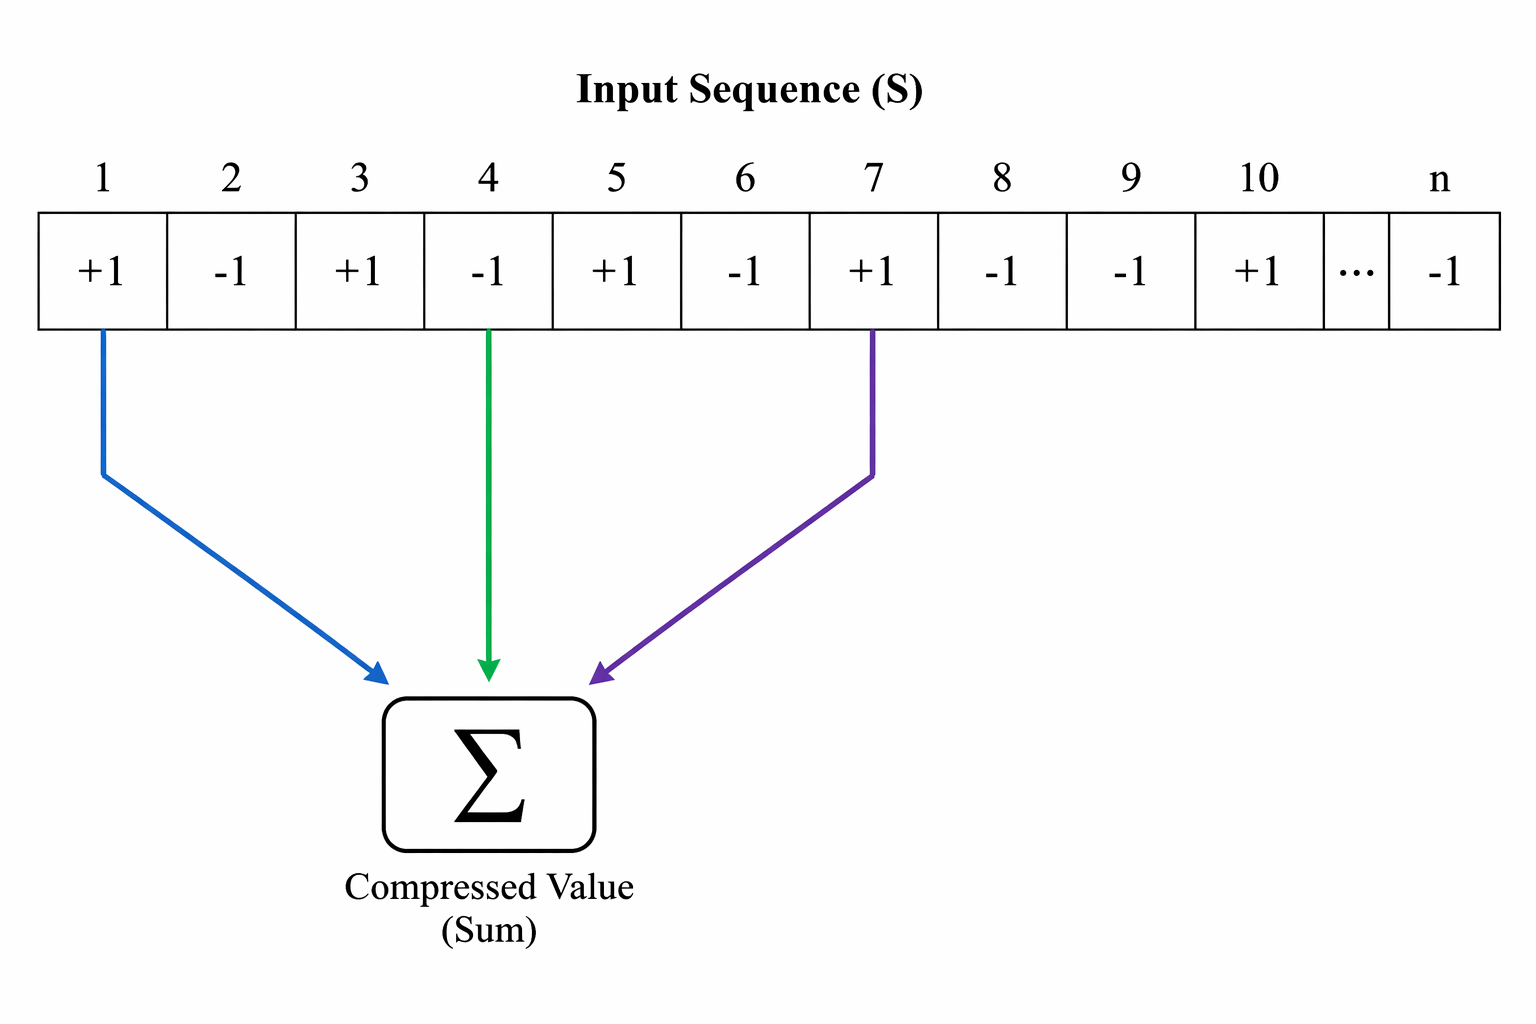
\includegraphics[width=0.75\linewidth]{compression_image.png}
    \caption{Representación visual del mapeo de compresión por un factor d=3. Los elementos binarios colapsan algebraicamente mediante sumas periódicas en un único elemento entero, reduciendo la dimensionalidad del problema original.}
    \label{fig:compression}
\end{figure}
    
\subsubsection*{Ejemplo 1: Compresión ilustrativa a pequeña escala ($\ell=9, d=3$)}

Para visualizar el mecanismo, imaginemos una secuencia arbitraria muy pequeña de longitud $\ell=9$. El factor de compresión es $d=3$, por lo que la secuencia comprimida tendrá una longitud $m = 9/3 = 3$.

Sea la secuencia original:
$$A = (+1, +1, -1, -1, +1, +1, -1, -1, -1)$$

Aplicando la fórmula, sumamos elementos separados por un salto de $m=3$ posiciones:
\begin{itemize}
    \item $A^{(3)}_0 = a_0 + a_3 + a_6 = (+1) + (-1) + (-1) = -1$
    \item $A^{(3)}_1 = a_1 + a_4 + a_7 = (+1) + (+1) + (-1) = +1$
    \item $A^{(3)}_2 = a_2 + a_5 + a_8 = (-1) + (+1) + (-1) = -1$
\end{itemize}

La secuencia resultante comprimida es $A^{(3)} = (-1, +1, -1)$. Se ha pasado de evaluar 9 variables binarias a evaluar un array de tan solo 3 variables enteras.

\subsubsection*{Ejemplo 2: El caso de estudio principal ($\ell=75, d=3$)}

Extrapolando este concepto a nuestro objetivo principal en el supercomputador, partimos de secuencias desconocidas $A$ y $B$ de longitud $\ell=75$. Aplicando $d=3$, obtenemos vectores comprimidos $A^{(3)}$ y $B^{(3)}$ de longitud $m=25$.

Esta compresión tiene una propiedad espectral fundamental: la densidad espectral de potencia (PSD) de las secuencias comprimidas preserva una relación proporcional con la secuencia original en las frecuencias correspondientes. Por tanto, el software no necesita buscar en el inabarcable espacio de $2^{150}$ combinaciones originales, sino que evalúa candidatos en el espacio de combinaciones de 25 elementos sobre el alfabeto $\{-3, -1, +1, +3\}$. 

Una vez que el algoritmo detecta un par comprimido $(A^{(3)}, B^{(3)})$ cuya PSD en el dominio frecuencial es compatible con la constante objetivo $2\ell + 2 = 152$, sabemos que es un candidato viable, y procedemos a su descompresión para verificar el Par de Legendre exacto.

\section{Historia de los pares de Legendre}

El estudio de secuencias con autocorrelación ideal tiene sus raíces en los problemas de diseño combinatorio del siglo XX. Aunque el nombre ''Pares de Legendre'' evoca al matemático Adrien-Marie Legendre debido al uso de los símbolos de residuos cuadráticos, su definición moderna en el contexto de procesamiento de señal es posterior.

Históricamente, la investigación se centró en encontrar secuencias únicas (como las secuencias de Barker), pero la demostración de su inexistencia para longitudes impares mayores que 13 motivó la búsqueda de \emph{pares} de secuencias complementarias. Investigadores como \cite{seberry1992hadamard} formalizaron la conexión entre estos pares y las Matrices de Hadamard, un problema abierto desde hace más de un siglo.

Recientemente, el trabajo de  \cite{kotsireas2021legendre} revitalizó el campo aplicando optimización computacional para longitudes $\ell$ divisibles por 3. Este TFG toma el relevo de dichos trabajos, proponiendo una modernización de las herramientas de búsqueda mediante paralelismo masivo y generación automática de código.

\section{Aplicaciones y logros de los pares de Legendre}

La relevancia de estas secuencias trasciende la teoría matemática pura; poseen aplicaciones prácticas directas en ingeniería moderna.

\subsection{Sistemas de radar y sonar}
En el diseño de ondas para radar, el objetivo fundamental es lograr una Función de Ambigüedad que se aproxime a un impulso ideal. La capacidad de discernir el eco de un objetivo frente al ruido depende de la Función de Autocorrelación Periódica (PAF) de la señal emitida.
\end{document}
Si transmitimos una secuencia $S$, buscamos que el lóbulo principal en el retardo $\tau = 0$ contenga toda la energía, y que los lóbulos laterales (\emph{sidelobes}) sean nulos para evitar objetivos fantasma. Los pares de Legendre son valiosos porque, al transmitirse en esquemas ortogonales complementarios, la suma de sus interferencias se cancela casi perfectamente:
$$ \text{PAF}_A(\tau) + \text{PAF}_B(\tau) = \begin{cases} 2\ell, & \tau \equiv 0 \pmod \ell \\ -2, & \tau \not\equiv 0 \pmod \ell \end{cases} $$
Esta propiedad de autocorrelación casi impulsiva maximiza la Relación Señal a Ruido (SNR), mejorando radicalmente la resolución espacial del radar y mitigando las interferencias de trayectos múltiples (\emph{multipath fading}) \cite{budivsin1991efficient}.

\begin{figure}[htb!]
    \centering
    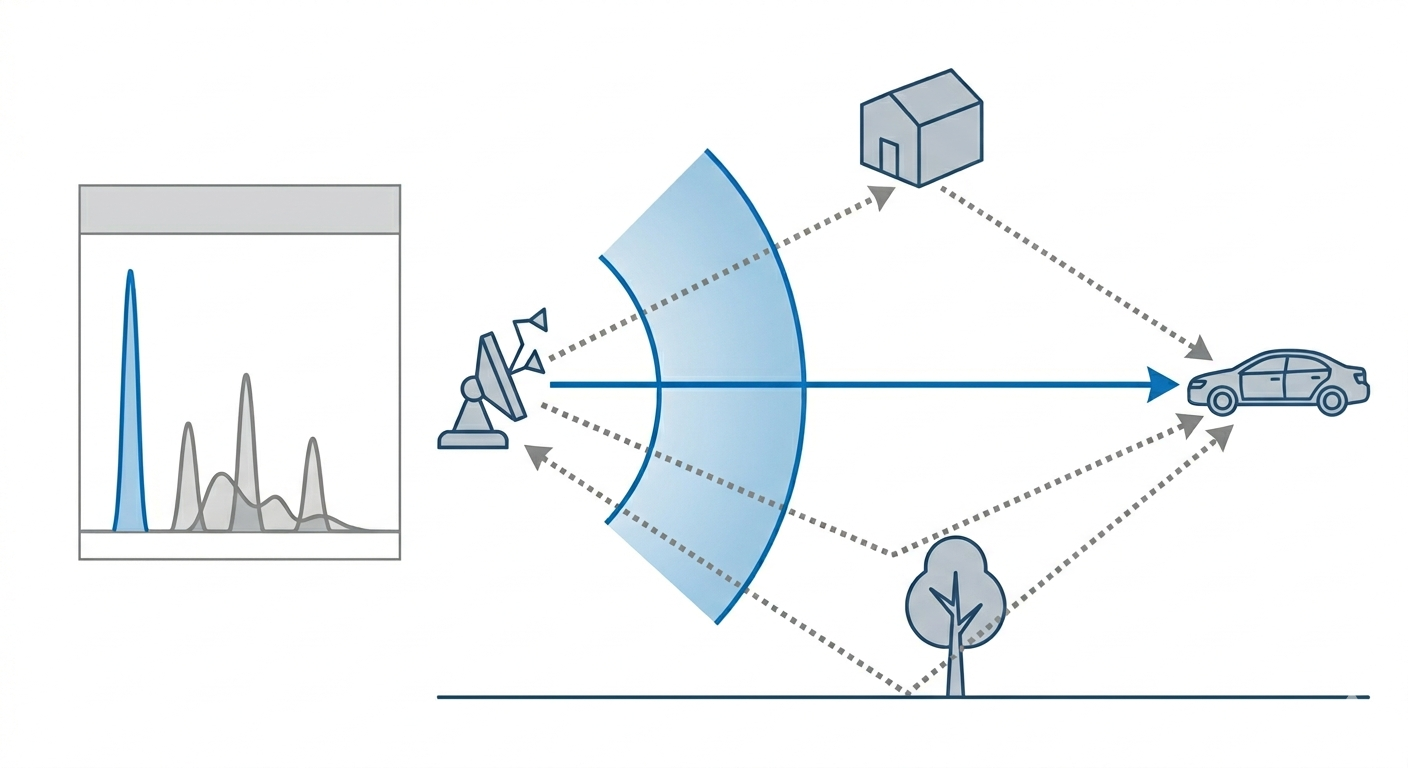
\includegraphics[width=0.85\linewidth]{radar_multipath.png}
    \caption{Visualización del fenómeno de desvanecimiento por trayectos múltiples (\emph{multipath fading}). La capacidad del receptor para aislar el pulso directo frente a los ecos parásitos depende críticamente de la autocorrelación de secuencias ortogonales como los pares de Legendre.}
    \label{fig:multipath}
\end{figure}

\subsection{Diseño de experimentos y matrices ortogonales}
En estadística experimental, las matrices ortogonales se utilizan para estudiar el efecto de múltiples variables de forma simultánea, garantizando que la varianza sea mínima y los efectos independientes. La estructura óptima para esto es la Matriz de Hadamard, una matriz cuadrada $H$ de orden $n$ con entradas en $\{-1, 1\}$ que satisface:
$$ H H^T = n I_n $$
donde $I_n$ es la matriz identidad. La construcción directa de estas matrices es un problema matemático abierto. Sin embargo, si existe un Par de Legendre $(A, B)$ de longitud $\ell$, se puede construir algebraicamente una Matriz de Hadamard de orden $n = 2\ell + 2$ utilizando la construcción de dos circulantes (\emph{two-circulant core construction}). Se forman matrices circulantes $C_A$ y $C_B$ a partir de los vectores $A$ y $B$, insertándolas en un bloque maestro estructurado que garantiza la ortogonalidad estricta entre todas las filas y columnas resultantes \cite{seberry1992hadamard}.

\begin{figure}[htb!]
    \centering
    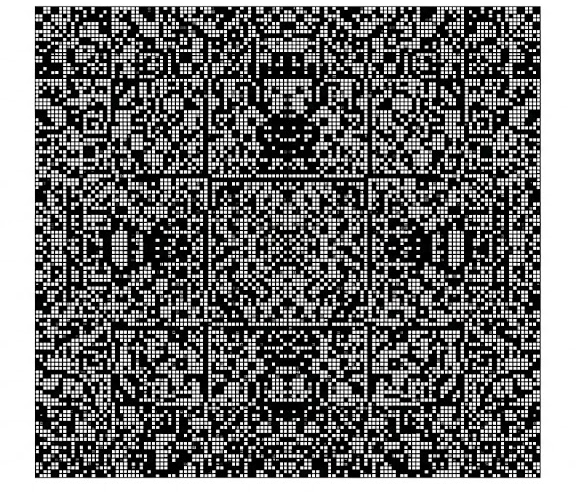
\includegraphics[width=0.6\linewidth]{hadamard_matrix.png}
    \caption{Representación gráfica de la estructura ortogonal de una matriz de Hadamard. El mapeo de secuencias de Legendre permite construir el núcleo (\emph{core}) de estas matrices para órdenes superiores.}
    \label{fig:hadamard}
\end{figure}

\subsection{Criptografía y secuencias pseudoaleatorias}
En sistemas de telecomunicaciones seguros, como el espectro ensanchado (Spread Spectrum) y los cifradores de flujo (\emph{stream ciphers}), es crucial que la señal portadora sea estadísticamente indistinguible del ruido blanco gaussiano para evitar la interceptación y el criptoanálisis.

Por el Teorema de Parseval, la energía total de una señal en el dominio del tiempo es igual a su energía en el dominio de la frecuencia. Un par de Legendre asegura una Densidad Espectral de Potencia (PSD) sumada estrictamente constante para todo componente frecuencial $k$:
$$ \text{PSD}_A(k) + \text{PSD}_B(k) = c $$
Esta uniformidad espectral (espectro plano) dota a las secuencias de Legendre de un alto nivel de entropía, baja predictibilidad lineal y un comportamiento cuasi-aleatorio perfecto, haciéndolas ideales como firmas digitales u ondas portadoras inmunes a ataques por análisis de frecuencia \cite{damgaard1988randomness}.

\subsection{Sistemas de posicionamiento satelital (GPS) y localización UWB}
El auge de los sistemas de localización, tanto en exteriores (sistemas satelitales GNSS/GPS) como en interiores mediante señales de radio de impulso ultraancho (IR-UWB), exige una precisión submétrica en el cálculo del Tiempo de Llegada (ToA) y la Diferencia de Tiempo de Llegada (TDoA). En estos entornos industriales o urbanos, las señales electromagnéticas se enfrentan a un canal hostil caracterizado por el desvanecimiento por trayectos múltiples (\emph{multipath fading}), donde los ecos de la señal rebotan en obstáculos y confunden al receptor \cite{cantabria2021positioning}.

Para mitigar este efecto y aislar la señal directa real, los sistemas modernos rechazan las modulaciones clásicas en favor del Acceso Múltiple por División de Código (CDMA) o modulaciones por posición de pulso combinadas con saltos temporales (TH-PPM). Es aquí donde los Pares de Legendre demuestran una utilidad excepcional. 

Al emplear estas secuencias combinatorias para modular los pulsos, se aprovecha su propiedad de autocorrelación casi ideal. El receptor, que conoce la secuencia de antemano, realiza una correlación cruzada con la señal entrante. Gracias a la estructura de Legendre, el pico de correlación en el retardo exacto $\tau = 0$ es agudo y destacadísimo, mientras que los ecos desplazados caen en lóbulos laterales nulos o mínimos. Esto permite identificar el instante exacto del impacto del pulso principal con precisión de picosegundos.

Adicionalmente, el uso de familias de secuencias pseudoaleatorias derivadas de Legendre asegura una baja correlación cruzada entre distintos transmisores. Esto soluciona dos problemas críticos del mercado actual del posicionamiento: 
\begin{itemize}
    \item \textbf{Escalabilidad:} Permite que decenas de etiquetas móviles (MUs) y puntos de acceso (APs) compartan el mismo ancho de banda sin colisiones destructivas.
    \item \textbf{Seguridad de capa física:} Previene ataques activos de interferencia (\emph{jamming}) y suplantación (\emph{spoofing} o ataques \emph{Early-Detection/Late-Commit}). Al ser el espectro de la señal estadísticamente indistinguible del ruido blanco para un interceptor que desconoce la secuencia, el atacante no puede inyectar energía maliciosa de manera coherente para alterar la estimación de distancia.
\end{itemize}

\section{Propiedades matemáticas fundamentales}

Para comprender la lógica implementada en el código desarrollado, es necesario formalizar las propiedades que nuestro algoritmo verifica. Un par de Legendre de longitud $\ell$ está formado por dos secuencias $A = \{a_i\}$ y $B = \{b_i\}$ con valores en $\{-1, +1\}$.

\subsection{Función de Autocorrelación Periódica (PAF)}
La condición en el dominio del tiempo exige que la suma de las autocorrelaciones de A y B sea una función delta (cero en todo punto salvo en el origen):
\[
\text{PAF}_A(k) + \text{PAF}_B(k) = \sum_{i=0}^{\ell-1} (a_i a_{i+k} + b_i b_{i+k}) = -2, \quad \forall k \neq 0 \pmod \ell
\]

\subsection{Densidad Espectral de Potencia (PSD)}
Verificar la PAF tiene una complejidad computacional de $O(\ell^2)$. Para acelerar el cálculo, trasladamos el problema al dominio de la frecuencia usando la Transformada Discreta de Fourier (DFT). La condición equivalente, y la que nuestro software verifica, es que la suma de las energías espectrales sea constante:
\[
|\text{DFT}_A(k)|^2 + |\text{DFT}_B(k)|^2 = 2\ell + 2, \quad \forall k
\]
Esta propiedad permite una verificación en tiempo $O(\ell)$ una vez calculada la DFT, siendo mucho más eficiente para el filtrado masivo de millones de candidatos por segundo.



La formulación en el dominio frecuencial establece que un par es válido si y solo si la suma de sus densidades espectrales es exactamente igual a la constante $2\ell + 2$ para cualquier frecuencia discreta $k$. Por ende, cualquier mínima desviación de este valor en una sola frecuencia descarta inmediatamente al candidato. Dado que esta evaluación debe realizarse para cada una de las trillones de combinaciones generadas, el cálculo repetitivo de las multiplicaciones complejas de la DFT se erige como el principal ''cuello de botella'' computacional del sistema. Optimizar el flujo de instrucciones de esta métrica es el objetivo primordial de la metaprogramación desarrollada.

\subsection{Análisis de Funciones Booleanas mediante la Transformada de Walsh-Hadamard}
En el ámbito de la criptografía, los Pares de Legendre y las secuencias de espectro plano están íntimamente ligados a la robustez de las funciones booleanas empleadas en S-boxes (para cifradores de bloque) y en combinadores de registros de desplazamiento (para cifradores de flujo). Una función booleana $f: \mathbb{F}_2^n \to \mathbb{F}_2$ debe exhibir la máxima no linealidad posible para frustrar el criptoanálisis lineal y diferencial.

La herramienta matemática estándar para desnudar y cuantificar cualquier linealidad oculta en estas funciones es la Transformada de Walsh-Hadamard (WHT). Conceptualmente, la WHT es el caso especial de la Transformada Discreta de Fourier sobre el grupo abeliano finito $\mathbb{F}_2^n$.

Para calcular el espectro de Walsh de una función, se multiplica su vector de verdad polarizado por una Matriz de Hadamard de orden $2^n$. Sin embargo, es un requisito matemático estricto que dicha matriz se genere exclusivamente mediante la \textbf{construcción de Sylvester}. Esta matriz se define de forma recursiva a través del producto tensorial de Kronecker:

$$ H_2 = \begin{pmatrix} 1 & 1 \\ 1 & -1 \end{pmatrix}, \quad H_{2^n} = H_2 \otimes H_{2^{n-1}} $$

La exigencia de usar la matriz de Sylvester radica en que su estructura indexada refleja perfectamente el espacio vectorial $\mathbb{F}_2^n$. Si se utilizara cualquier otra matriz de Hadamard isomórfica (generada por métodos de Paley, Williamson o secuencias aleatorias), el espectro resultante mostraría comportamientos no aleatorios y sesgos estructurales que destruirían el análisis, ya que las filas de la matriz no se corresponderían con las formas lineales canónicas del espacio de entrada.

Al aplicar la Transformada de Walsh-Hadamard de Sylvester, obtenemos un perfil que mide la correlación exacta entre nuestra función booleana y todas las funciones afines posibles. Por el Teorema de Parseval, la suma de los cuadrados de estos coeficientes de Walsh es constante. Cuando una función minimiza esta correlación de manera uniforme, su espectro de Walsh es completamente plano, tomando únicamente los valores límite $\pm 2^{n/2}$. A estas funciones de máxima no linealidad se les denomina \emph{funciones Bent} \cite{rothaus1976bent, pommerening2014fourier}.

La búsqueda de Pares de Legendre está profundamente anclada a este fenómeno algebraico. La planitud espectral en el dominio booleano (funciones Bent) es el análogo directo de la condición de Densidad Espectral de Potencia (PSD) constante que nuestro software verifica algorítmicamente. Encontrar soluciones óptimas en la teoría de Legendre proporciona vectores base directos para sintetizar funciones con inmunidad teórica máxima frente al criptoanálisis.


\section{Metodología y Herramientas de Desarrollo}

Para abordar un problema de esta envergadura computacional, fue necesario establecer un marco metodológico estricto y seleccionar cuidadosamente la pila tecnológica (\emph{tech stack}).

\subsection{Metodología en Cascada (Waterfall)}
A diferencia de proyectos de software comercial donde los requisitos cambian constantemente (lo que favorecería metodologías Ágiles), este problema matemático está rígidamente definido desde el principio. Por ello, se optó por un enfoque en \textbf{Cascada}. 

Cada fase de desarrollo se concibió para identificar y solucionar el cuello de botella de la fase anterior:
\begin{enumerate}
    \item \textbf{Fase Matemática:} Definición teórica del problema y reducción algebraica mediante cosets ciclotómicos.
    \item \textbf{Fase de Prototipado Secuencial:} Implementación de algoritmos base en C que escriben/leen en disco para validar la correctitud.
    \item \textbf{Fase de Refinamiento Algorítmico:} Transición a algoritmos de Búsqueda en Profundidad (DFS) en memoria con estrategias de poda (pruning) para evitar el colapso por Entrada/Salida (I/O).
    \item \textbf{Fase de Paralelización y Metaprogramación:} Generación de código a medida y despliegue masivo (OpenMP/Slurm) para romper los límites de tiempo del superordenador.
\end{enumerate}

\begin{figure}[htb!]
    \centering
    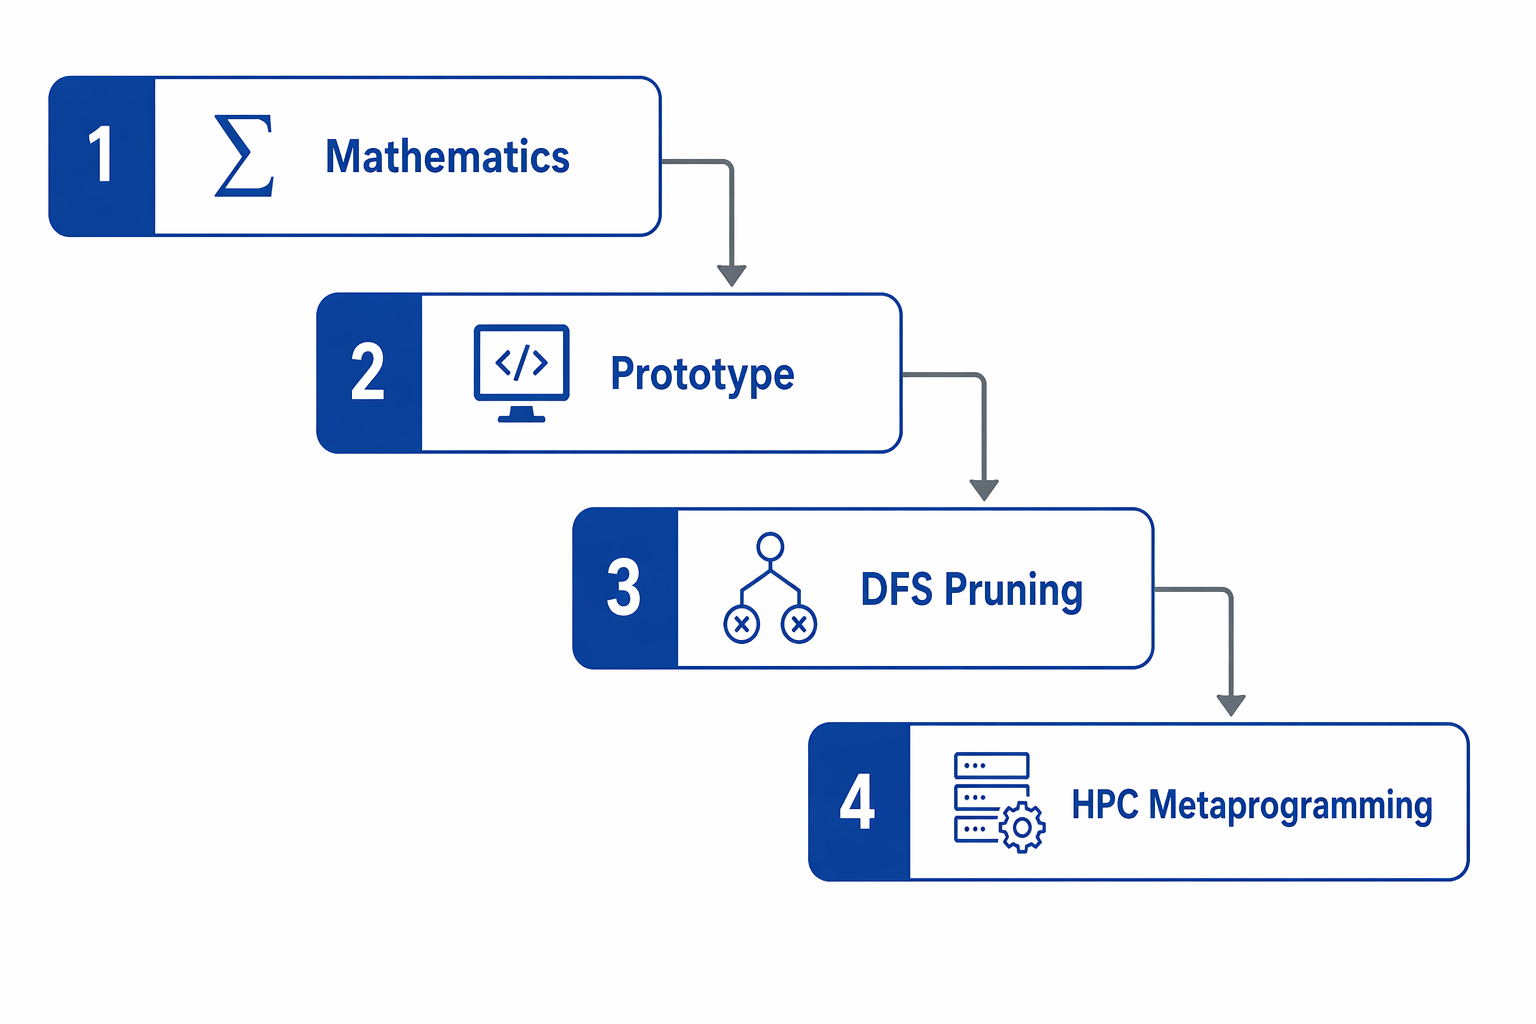
\includegraphics[width=0.75\linewidth]{cascade_image.png}
    \caption{Metodología de desarrollo secuencial (Cascada). Cada etapa del proyecto fue diseñada iterativamente para aislar, analizar y eliminar los cuellos de botella computacionales identificados en la fase previa.}
    \label{fig:cascade}
\end{figure}

\subsection{Herramientas y Decisiones Arquitectónicas}
El entorno de ejecución fue el Supercomputador Altamira (IFCA). Las herramientas seleccionadas fueron:
\begin{itemize}
    \item \textbf{Lenguajes C y C++:} Elegidos por su nula sobrecarga en tiempo de ejecución, acceso directo a memoria y madurez de sus compiladores para vectorización.
    \item \textbf{GCC (GNU Compiler Collection):} Utilizando las \emph{flags} \texttt{-O3 -march=native} para obligar al compilador a usar las instrucciones SIMD específicas de los procesadores del clúster.
    \item \textbf{OpenMP vs. MPI:} Se evaluó el uso de MPI (Message Passing Interface) para paralelizar la búsqueda entre múltiples nodos. Sin embargo, \textbf{se descartó a favor de OpenMP + Slurm Arrays}. El problema de búsqueda de Legendre es un problema \emph{embarrassingly parallel} (vergonzosamente paralelo) sin necesidad de que los nodos se comuniquen entre sí. MPI habría añadido una complejidad innecesaria y un sobrecoste de comunicación (\emph{network overhead}) contraproducente. La paralelización híbrida (OpenMP para hilos dentro de un nodo, y Slurm para distribuir entre nodos de forma estanca) resultó ser la aproximación óptima.
    \item \textbf{Sistema de Colas Slurm:} Fundamental para la gestión de trabajos mediante \emph{Job Arrays}, eludiendo los límites de tiempo de la plataforma \cite{yoo2003slurm}.
\end{itemize}


% ==============================================================================
% CAPÍTULO 2: DESARROLLO
% ==============================================================================
\chapter{Desarrollo e Innovaciones Algorítmicas}

El núcleo de este Trabajo de Fin de Grado reside en la paulatina evolución de la arquitectura del software, concebida para doblegar la intratabilidad computacional de los espacios de búsqueda masivos asociados a los pares de Legendre. Este capítulo traza la hoja de ruta integral del proyecto, detallando el progreso secuencial desde la formulación de los algoritmos matemáticos iniciales hasta el despliegue de un generador de código de alto rendimiento en la infraestructura del supercomputador Altamira.

La resolución de un espacio de dimensionalidad exponencial no puede abordarse mediante un único incremento de fuerza bruta, sino que requiere una orquestación de técnicas transversales en múltiples niveles de abstracción informática y matemática. En primer lugar, se expondrá la base teórica de la reducción dimensional mediante órbitas de equivalencia ciclotómica, estableciendo el cimiento algebraico indispensable sobre el cual operan todos los algoritmos posteriores. 

A continuación, se documentará la evolución iterativa del motor de búsqueda. Se analizará el fracaso de las implementaciones primigenias, cuyo rendimiento se veía asfixiado por los severos cuellos de botella de entrada y salida (I/O) en el disco físico, y se justificará la transición hacia un modelo dinámico de Búsqueda en Profundidad (DFS) ejecutado íntegramente en la memoria principal. En este punto, se detallará cómo la inyección de heurísticas de poda matemática y el rediseño de las estructuras de datos para aprovechar operaciones a nivel de bit (paralelismo SWAR intra-registro) permitieron al software descartar billones de ramas estériles sin la necesidad de evaluarlas computacionalmente.

Aun con estas mejoras, la optimización algorítmica clásica posee un límite asintótico inquebrantable frente a la explosión combinatoria. Por ello, la segunda mitad del capítulo se adentra en el cambio de paradigma hacia la computación distribuida y la persistencia de datos probabilística. Se expondrá la integración de Filtros de Bloom para orquestar una estrategia \emph{Meet-in-the-Middle} capaz de alterar la complejidad temporal del problema aislando sus subespacios, logrando contener el colapso teórico de la memoria RAM. 


Finalmente, se coronará el desarrollo detallando la arquitectura de metaprogramación: la creación de un sistema matriz capaz de transcribir su propio código fuente en C++, desenrollando bucles y eliminando la latencia de las ramificaciones condicionales para acoplarse de forma nativa a las instrucciones vectoriales del procesador anfitrión. Este recorrido ilustra, paso a paso, la metamorfosis de un problema analítico de matemáticas discretas en un desafío integral de ingeniería de software, arquitecturas superescalares y orquestación de clústers de supercomputación.

\section{Reducción Algebraica: Cosets Ciclotómicos}

En lugar de iterar por cada bit individual de una secuencia de longitud $\ell$, las propiedades de simetría de las secuencias de Legendre permiten agrupar los índices en clases de equivalencia bajo multiplicación por 2, denominadas \textbf{Cosets Ciclotómicos}. Formalmente, para un índice $s \in \{0, 1, \dots, \ell-1\}$, el coset ciclotómico $C_s$ módulo $\ell$ se define como la órbita generada al multiplicar iterativamente por 2:

$$ C_s = \{ s \cdot 2^i \pmod{\ell} \mid i \in \mathbb{N} \} $$

El tamaño de cada órbita está determinado por el orden multiplicativo de 2 módulo $\ell/\text{mcd}(s, \ell)$. Esta operación matemática divide el dominio discreto original en conjuntos completamente disjuntos. La principal restricción algebraica de este método dicta que, si la secuencia $(a_0, a_1, \dots, a_{\ell-1})$ es un candidato válido, entonces para cualquier par de índices $j, k \in C_s$, se cumple de manera estricta que $a_j = a_k$. En otras palabras, la secuencia es invariante ante una decimación diádica. Esta propiedad colapsa la dimensionalidad del problema: ya no decidimos el valor de $\ell$ variables independientes, sino el valor de un número sustancialmente menor de cosets, actuando cada uno como un bloque atómico.

Para el caso objetivo $\ell=75$, la partición del anillo $\mathbb{Z}_{75}$ genera exactamente 45 cosets distintos, cada uno con una cardinalidad que varía dependiendo de la estructura multiplicativa del grupo subyacente (en este caso, tamaños típicos de 1, 2, 4 o 20 elementos). Matemáticamente, esto significa que el espacio de búsqueda original de $2^{75}$ combinaciones se proyecta sobre un subespacio isomórfico de $2^{45}$. Esta reducción matemática elimina redundancias intrínsecas y reduce el exponente de complejidad en 30 magnitudes completas. 

A pesar del extraordinario recorte dimensional, evaluar empíricamente $2^{45}$ candidatos (aproximadamente $3.5 \times 10^{13}$ evaluaciones) sigue siendo un reto masivo que desborda las capacidades de la fuerza bruta lineal. Para ilustrar la dificultad, a una velocidad sostenida de 100,000 iteraciones por segundo por núcleo computacional, verificar el espacio reducido consumiría más de 11 años ininterrumpidos en hardware estándar, lo cual exige obligatoriamente la transición hacia estrategias algorítmicas avanzadas y podas.

\begin{figure}[htb!]
    \centering
    \framebox{\begin{minipage}{0.9\textwidth}
        \centering
        \vspace{4cm}
        \textcolor{red}{\textbf{[IMAGEN SUGERIDA 2]}} \\
        \textcolor{red}{Diagrama de Metodología Cascada.} \\
        \textcolor{red}{Dibuja 4 escalones descendentes que ilustren las fases descritas arriba: Matemáticas $\rightarrow$ Prototipo $\rightarrow$ Poda DFS $\rightarrow$ Paralelismo HPC.}
        \vspace{4cm}
    \end{minipage}}
    \caption{Metodología de desarrollo en Cascada orientada a la eliminación progresiva de cuellos de botella.}
    \label{fig:waterfall}
\end{figure}

\subsection{Herramientas y Decisiones Arquitectónicas}
El entorno de ejecución fue el Supercomputador Altamira (IFCA). Las herramientas seleccionadas fueron:
\begin{itemize}
    \item \textbf{Lenguajes C y C++:} Elegidos por su nula sobrecarga en tiempo de ejecución, acceso directo a memoria y madurez de sus compiladores para vectorización.
    \item \textbf{GCC (GNU Compiler Collection):} Utilizando las \emph{flags} \texttt{-O3 -march=native} para obligar al compilador a usar las instrucciones SIMD específicas de los procesadores del clúster.
    \item \textbf{OpenMP vs. MPI:} Se evaluó el uso de MPI (Message Passing Interface) para paralelizar la búsqueda entre múltiples nodos. Sin embargo, \textbf{se descartó a favor de OpenMP + Slurm Arrays}. El problema de búsqueda de Legendre es un problema \emph{embarrassingly parallel} (vergonzosamente paralelo) sin necesidad de que los nodos se comuniquen entre sí. MPI habría añadido una complejidad innecesaria y un sobrecoste de comunicación (\emph{network overhead}) contraproducente. La paralelización híbrida (OpenMP para hilos dentro de un nodo, y Slurm para distribuir entre nodos de forma estanca) resultó ser la aproximación óptima.
    \item \textbf{Sistema de Colas Slurm:} Fundamental para la gestión de trabajos mediante \emph{Job Arrays}, eludiendo los límites de tiempo de la plataforma.
\end{itemize}


% ==============================================================================
% CAPÍTULO 2: DESARROLLO
% ==============================================================================
\chapter{Desarrollo e Innovaciones Algorítmicas}

El núcleo de este TFG reside en la paulatina evolución del software para lograr verificar espacios de búsqueda masivos. Este capítulo detalla el progreso desde los algoritmos matemáticos iniciales hasta el despliegue del generador optimizado.

\section{Reducción Algebraica: Cosets Ciclotómicos}

En lugar de iterar por cada bit individual de una secuencia de longitud $N$, las propiedades matemáticas de las secuencias de Legendre permiten agrupar los índices en conjuntos invariantes llamados \textbf{Cosets Ciclotómicos}.

Si un bit cambia en un índice perteneciente a un coset, todos los demás bits de ese mismo coset deben obligatoriamente tener el mismo valor. Esto reduce drásticamente las variables de decisión. Por ejemplo, para $N=75$, la longitud se descompone en 45 cosets distintos. Esto significa que el espacio de búsqueda baja de un inexplorable $2^{75}$ a un más tratable $2^{45}$.

\begin{figure}[H]
    \centering
    \framebox{\begin{minipage}{0.9\textwidth}
        \centering
        \vspace{4.5cm}
        \textcolor{red}{\textbf{[IMAGEN SUGERIDA 3]}} \\
        \textcolor{red}{Ejemplo visual de un Coset.} \\
        \textcolor{red}{Muestra un array lineal y señala cómo los índices 1, 2, 4, 8 (un coset de potencias de 2, por ejemplo) están obligados a valer lo mismo (+1 o -1 a la vez).}
        \vspace{4.5cm}
    \end{minipage}}
    \caption{Ejemplo de reducción de dimensionalidad agolpando índices en Cosets Ciclotómicos.}
    \label{fig:coset_example}
\end{figure}


\section{Evolución del Software: De la I/O a la Búsqueda en Profundidad}

El desarrollo se estructuró en versiones progresivas del código (\texttt{main\_txt.c}, \texttt{main-1.c}, \texttt{main.c}), cada una superando las deficiencias de la anterior.

\subsection{Fase 1: Fuerza Bruta sobre Cosets y Archivos Intermedios}
El código inicial (\texttt{main\_txt.c}) aplicaba el concepto de los cosets generando exhaustivamente combinaciones, calculando sus espectros, y escribiendo todo en archivos de texto plano masivos (ej. \texttt{comp\_dft\_cosets.txt}). 

Posteriormente, la función \texttt{buscar\_pares\_complementarios} leía las PSDs y buscaba combinaciones que sumaran el objetivo ($2N+2$). Finalmente se empleaba la función \texttt{find\_matches\_files} para cruzar los archivos y encontrar los pares.

\begin{lstlisting}[caption={Fragmento de la lógica inicial de cruce de ficheros (\texttt{main\_txt.c})}]
// Bucle anidado de fuerza bruta comparando todas las PSDs leidas
for (size_t i = 0; i < total; i++) {
    for (size_t j = i + 1; j < total; j++) {
        if ((col1[i] + col1[j]) == objetivo) {
            fprintf(f_out, ''%s\n%s\n\n'', secuencias[i], secuencias[j]);
=======
    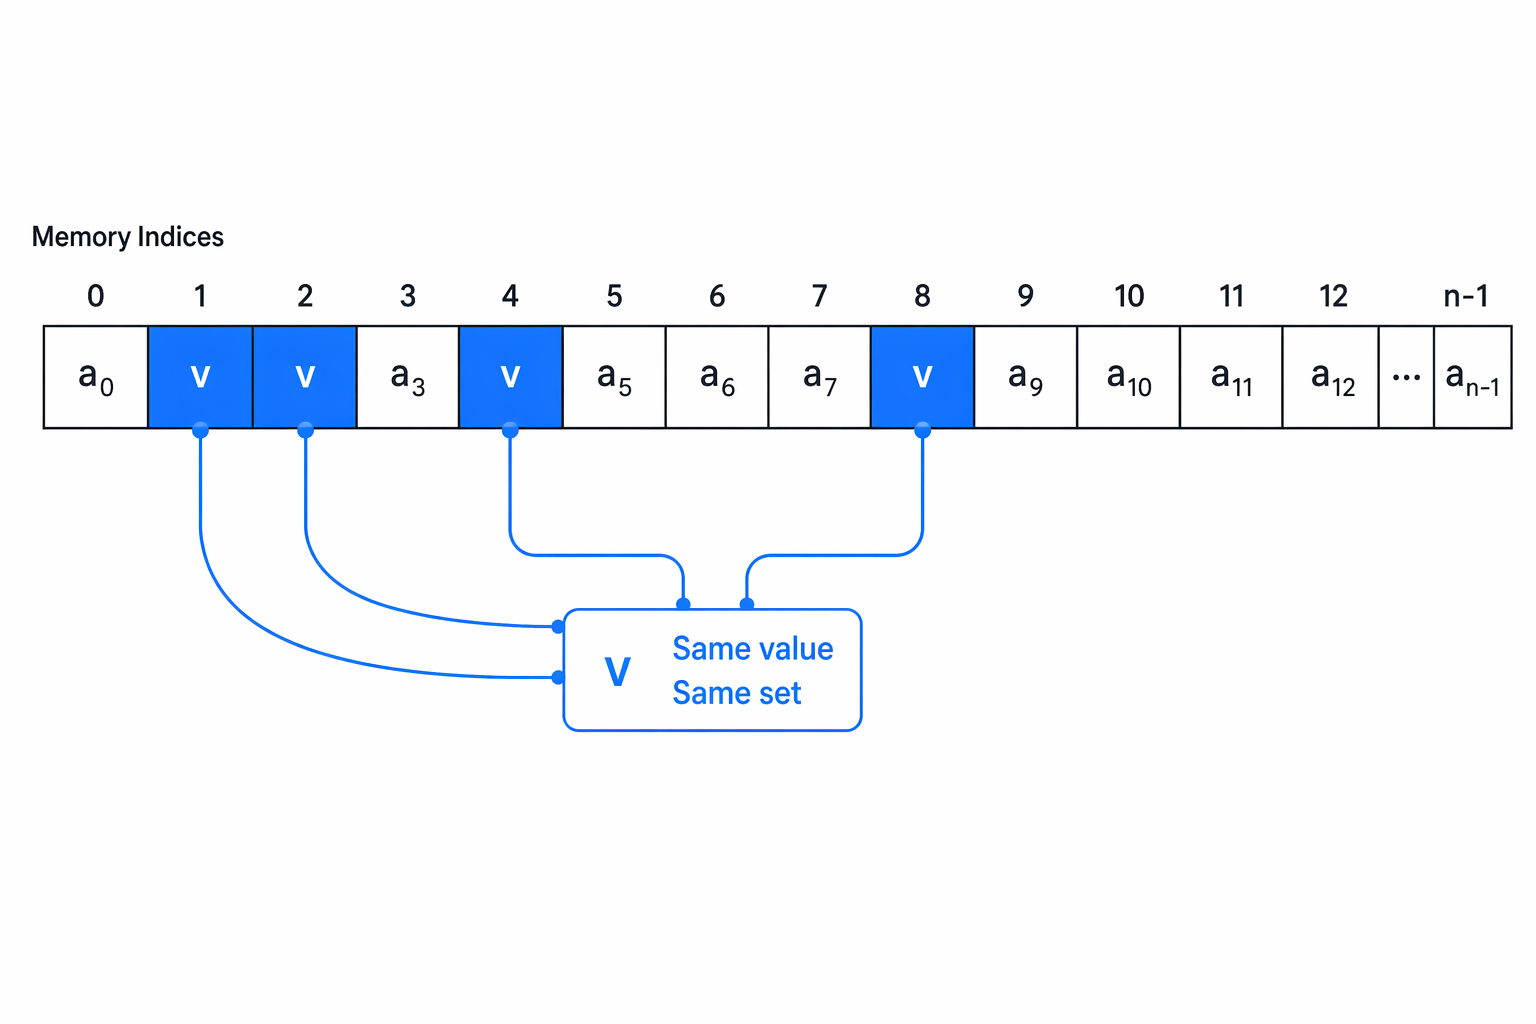
\includegraphics[width=0.75\linewidth]{cyclotomic_coset_image.png}
    \caption{Agrupación de índices mediante cosets ciclotómicos. La restricción algebraica que obliga a múltiples posiciones del array a compartir el mismo valor reduce drásticamente la entropía del espacio de búsqueda.}
    \label{fig:cosets}
\end{figure}

\section{Evolución del Software: De la I/O a la Búsqueda en Profundidad}

El desarrollo se estructuró en versiones progresivas del código (\texttt{main\_txt.c}, \texttt{main-1.c}, \texttt{main.c}), cada una superando empírica y arquitectónicamente las deficiencias y cuellos de botella aislados en la anterior.

\subsection{Fase 1: Fuerza Bruta sobre Cosets y Archivos Intermedios}
El código inicial (\texttt{main\_txt.c}) operaba bajo una arquitectura estrictamente secuencial y altamente acoplada al sistema de archivos. Aplicaba el concepto de los cosets generando exhaustivamente combinaciones mediante bucles iterativos, calculando sus espectros, y escribiendo la totalidad de los datos resultantes en archivos de texto plano masivos (ej. \texttt{comp\_dft\_cosets.txt}). 

Posteriormente, la función \texttt{buscar\_pares\_complementarios} actuaba como una segunda etapa aislada. Leía las PSDs almacenadas en disco y ejecutaba un recorrido de orden cuadrático comparando cada registro para buscar combinaciones que sumaran el objetivo exacto ($2N+2$). Finalmente, se empleaba la función \texttt{find\_matches\_files} para cruzar los archivos resultantes y mapear las posiciones con las secuencias originales correspondientes.

\begin{lstlisting}[caption={Fragmento de la lógica inicial de cruce de ficheros}]
for (size_t i = 0; i < total; i++) {
    for (size_t j = i + 1; j < total; j++) {
        if ((col1[i] + col1[j]) == objetivo) {
            fprintf(f_out, "%s\n%s\n\n", secuencias[i], secuencias[j]);
>>>>>>> origin/overleaf-2026-05-17-1603
            encontrados++;
        }
    }
}
\end{lstlisting}

<<<<<<< HEAD
\textbf{El problema:} Aunque matemáticamente correcto, este enfoque colapsaba rápidamente. El cuello de botella no era la CPU, sino el I/O (lectura/escritura) del disco duro del servidor, haciendo imposible explorar secuencias largas.

\subsection{Fase 2: Búsqueda en Profundidad (DFS) y Podas (Pruning)}
Para solucionar el colapso del disco, el código evolucionó a \texttt{main-1.c}, abandonando la escritura masiva a favor de un algoritmo de Búsqueda en Profundidad (DFS) ejecutado enteramente en memoria RAM.

En lugar de generar todas las combinaciones ($2^{45}$) y evaluarlas luego, el algoritmo construye la secuencia coset por coset (descendiendo por niveles del árbol DFS). La innovación crítica aquí es la introducción de las \textbf{Podas (Bounds)}.

Antes de asignar un valor (`0` o `1`) al siguiente coset, la función \texttt{check\_bound} calcula un límite teórico. Si matemáticamente se demuestra que la rama actual del árbol nunca podrá cumplir la condición PSD objetivo (independientemente de los cosets restantes), el algoritmo poda la rama entera.

\begin{lstlisting}[caption={Lógica de poda (pruning) durante la exploración DFS (\texttt{main-1.c})}, label={lst:pruning}]
bool check_bound(DFSContext *ctx) {
    // Verificaciones lineales previas
    bool result = is_less_than_candidates(ctx, 1) && is_less_than_candidates(ctx, 0);
    if (!result) return false;
    
    double max_lower_bound = 0.0;
    // Evaluacion del limite espectral
    for (int j = 1; j < ctx->spectrum_size; j++) {
        double current_abs = cabs(ctx->current_dft[j]);
        double lower_bound_psd = pow(fmax(0.0, current_abs - ctx->current_bound[j]), 2.0);
        if (lower_bound_psd > max_lower_bound) {
            max_lower_bound = lower_bound_psd;
        }
    }
    // Si el limite minimo ya supera el umbral, la rama se poda
    return max_lower_bound <= ctx->threshold; 
}
\end{lstlisting}

Esta técnica evitó evaluar billones de combinaciones inútiles, acelerando drásticamente el proceso.

\begin{figure}[H]
    \centering
    \framebox{\begin{minipage}{0.8\textwidth}
        \centering
        \vspace{4.5cm}
        \textcolor{red}{\textbf{[IMAGEN SUGERIDA 4]}} \\
        \textcolor{red}{Árbol de Decisión DFS con Podas.} \\
        \textcolor{red}{Dibuja un árbol binario. Muestra cómo al llegar a un nodo intermedio, la evaluación \texttt{check\_bound} devuelve ''Falso'' y toda la sub-rama debajo de ese nodo se tacha con una 'X' roja, simbolizando la poda.}
        \vspace{4.5cm}
    \end{minipage}}
    \caption{Efecto de la poda matemática en la reducción de ramas exploradas en el árbol DFS.}
    \label{fig:dfs_pruning}
\end{figure}

\subsection{Fase 3: El Estado del Arte (Bitsets y Ordenación Heurística)}
La versión definitiva en C (\texttt{main.c}) refinó el DFS para operar bajo principios de Alto Rendimiento:

\textbf{1. Estructuras Bitset para Filtrado Rápido:} 
En vez de recorrer arrays enteros con bucles \texttt{for}, se implementaron matrices de bits (`ge_bitsets`, `le_bitsets`). Estas estructuras permiten procesar 64 estados de candidatos en una sola instrucción de reloj usando operaciones nativas de CPU (`AND`, `OR` y `__builtin_popcountll`).

\begin{lstlisting}[caption={Filtrado masivo mediante operaciones de bits nativas de CPU (\texttt{main.c})}]
// ... dentro de exists_candidate_in_range_bitset ...
int count = 0;
for (size_t w = 0; w <= last_word; w++) {
    // Resolucion de limites operando 64 secuencias simultaneamente
    uint64_t bits = ge[j][l][w] & le[j][u][w];
    
    // Conteo optimizado en hardware de los bits a '1'
    count += __builtin_popcountll((unsigned long long)bits);
}
if (count == 0) return false; // Poda inmediata
\end{lstlisting}

\textbf{2. Reordenación Heurística de Cosets:} 
La eficacia de un algoritmo DFS depende de ''equivocarse rápido''. Si podamos ramas en el nivel 2, ahorramos mucho más tiempo que si podamos en el nivel 40. La función \texttt{reorder\_cosets\_by\_candidate\_pairs} analiza la restricción que impone cada coset y reorganiza el árbol dinámicamente, evaluando primero las decisiones más críticas. Esto maximiza la eficiencia de la poda descrita en el Código \ref{lst:pruning}.


\section{Reducción de Complejidad Extrema: Filtros de Bloom y Estrategia Meet-in-the-Middle}

A pesar de los avances con DFS y podas, el crecimiento de la complejidad dictaminaba la necesidad de un cambio de paradigma para secuencias grandes. El problema original obliga a evaluar $A$ contra $B$ en bucles anidados, produciendo una complejidad de $O(N_A \times N_B)$.

Sabemos que la condición de éxito es:
$$PSD_A(s) + PSD_B(s) = 2\ell + 2$$
Lo que significa que, si fijamos una secuencia $A$, sabemos de antemano exactamente qué PSD necesita tener $B$:
$$PSD_{B\_buscado}(s) = 2\ell + 2 - PSD_A(s)$$

Si pudiéramos guardar todas las secuencias deseadas en memoria, podríamos calcular $B$ una sola vez y consultar si existe. Esto es una estrategia \textbf{Meet-in-the-Middle}, que reduce la complejidad a $O(N_A + N_B)$. Sin embargo, almacenar trillones de perfiles espectrales colapsaría la memoria RAM de cualquier nodo del Altamira.

La solución arquitectónica propuesta en este trabajo es el uso de un \textbf{Filtro de Bloom} (Bloom Filter).

\begin{figure}[H]
    \centering
    \framebox{\begin{minipage}{0.9\textwidth}
        \centering
        \vspace{5cm}
        \textcolor{red}{\textbf{[IMAGEN SUGERIDA 5]}} \\
        \textcolor{red}{Estrategia Meet-in-the-Middle con Bloom Filter.} \\
        \textcolor{red}{Izquierda: ''Espacio Secuencias A'' inyectando hashes en un array de bits (Bloom Filter). Derecha: ''Espacio Secuencias B'' comprobando si su hash coincide con los bits del filtro en el centro.}
        \vspace{5cm}
    \end{minipage}}
    \caption{El Filtro de Bloom actúa como puente en la memoria RAM, permitiendo la estrategia Meet-in-the-Middle sin colapsar el sistema.}
    \label{fig:bloom_filter}
\end{figure}

Un Filtro de Bloom es una estructura de datos probabilística. Mediante el uso de múltiples funciones \textit{hash} (por ejemplo, el algoritmo `FNV-1a`), ''comprime'' la existencia de un candidato en unos pocos bits. Su ventaja radica en que tiene \textbf{cero falsos negativos} (si dice que $B$ no sirve, es seguro que no sirve) y un porcentaje ínfimo de falsos positivos (verificados a posteriori), requiriendo apenas unos megabytes de memoria para gestionar billones de combinaciones.

\begin{lstlisting}[caption={Generación de la función Hash inyectada en el código para el Filtro de Bloom}, label={lst:bloom_hash}]
// Funcion Hash ultrarrapida inyectada por el metaprograma
inline uint64_t hash_array(int* arr, int len, uint64_t seed) {
    uint64_t hash = 14695981039346656037ULL + seed;
    for(int i = 0; i < len; i++) {
        hash ^= (uint64_t)arr[i];
        hash *= 1099511628211ULL;
    }
    return hash;
}
\end{lstlisting}

\section{Estrategia de Metaprogramación: El Generador en C++}

Para cohesionar todas las optimizaciones matemáticas, el paralelismo OpenMP, los Filtros de Bloom y la necesidad de vectorización por CPU, se desarrolló la herramienta definitiva: el \textbf{Generador de Buscadores}.

El generador es una aplicación en C++ que no busca pares de Legendre directamente, sino que \emph{escribe el código fuente} en C++ de un buscador optimizado para una longitud $\ell$ determinada.

\begin{figure}[H]
    \centering
    %\begin{tcolorbox}[colback=blue!5!white,colframe=blue!75!black,title=Flujo de Metaprogramación]
    \centering
    \textbf{1. Input:} $\ell=75$. \\
    $\downarrow$ \\
    \textbf{2. Generación:} \texttt{generador\_de\_generadores.cpp} calcula simbólicamente raíces y genera bucles y Bloom Filters a medida. \\
    $\downarrow$ \\
    \textbf{3. Código Fuente:} Se crea \texttt{compress.75.cpp} 100\% plano y \emph{hardcoded}. \\
    $\downarrow$ \\
    \textbf{4. Compilación HPC:} \texttt{g++ -O3 -march=native}. \\
    $\downarrow$ \\
    \textbf{5. Despliegue:} Ejecución en Lotes vía Slurm.
=======
\textbf{El problema:} Aunque matemáticamente correcto, este enfoque colapsaba rápidamente al escalar la dimensión de $\ell$. La experimentación demostró que el cuello de botella crítico no residía en la capacidad de la Unidad Central de Procesamiento (CPU) para resolver la Transformada de Fourier, sino en la limitación física de \textbf{Entrada/Salida (I/O) del disco duro}. Escribir y leer iterativamente cadenas de caracteres desencadenaba un fenómeno de latencia extrema (\emph{I/O Wait}), saturando el ancho de banda del bus SATA o PCIe. Además, la carga térmica y de llamadas al sistema (\emph{syscalls} como \texttt{fprintf}) hacían imposible explorar secuencias largas en tiempos computacionales razonables.

\begin{figure}[htb!]
    \centering
    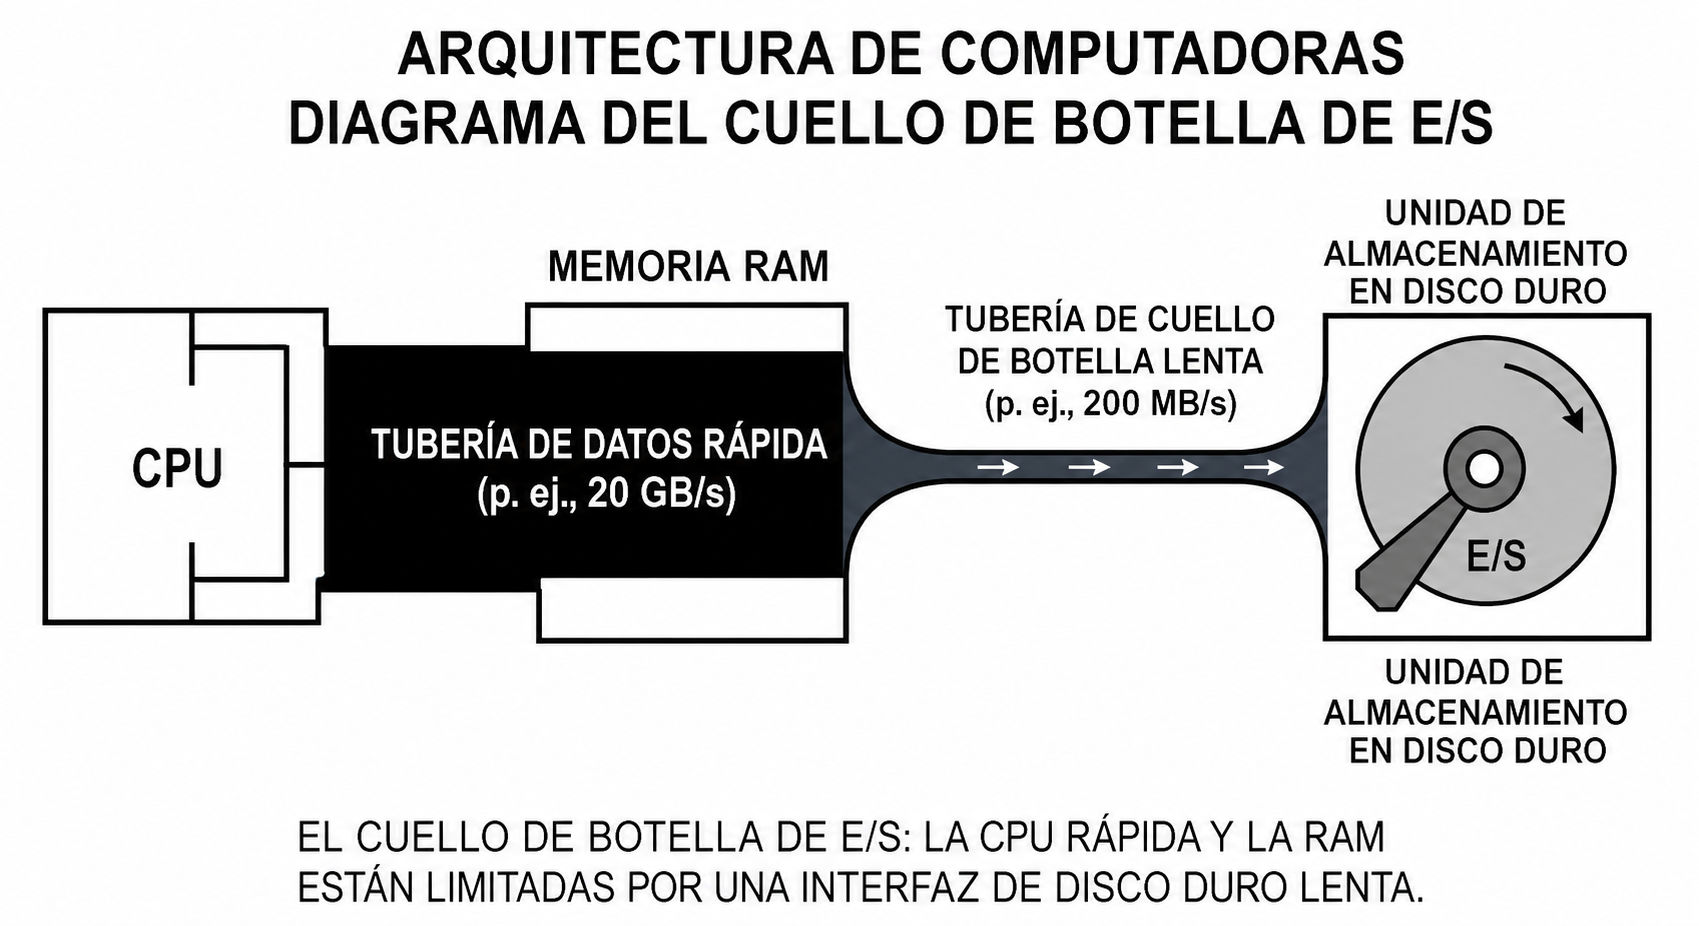
\includegraphics[width=0.8\linewidth]{io_bottleneck.png}
    \caption{Esquema del cuello de botella de Entrada/Salida (I/O). El rendimiento algorítmico de la Fase 1 se vio severamente estrangulado por la latencia del bus de almacenamiento físico, forzando la migración a un modelo in-memory.}
    \label{fig:io_bottleneck}
\end{figure}

\subsection{Fase 2: Búsqueda en Profundidad (DFS) y Podas (Pruning)}
Para solucionar el colapso del disco y suprimir por completo la dependencia del subsistema I/O, el código evolucionó a \texttt{main-1.c}, abandonando la escritura masiva a favor de un algoritmo algorítmicamente más inteligente: una Búsqueda en Profundidad (DFS) ejecutada íntegramente en memoria RAM.

En lugar de generar todas las combinaciones posibles en bloque ($2^{45}$ conjuntos estáticos) y evaluarlas de forma diferida, el algoritmo construye la secuencia elemento a elemento, descendiendo secuencialmente por niveles del árbol DFS asimilado a los índices de los cosets. La innovación crítica en esta fase es la introducción del mecanismo dinámico de \textbf{Podas (Bounds)}.

Antes de descender al siguiente nivel del árbol de exploración para asignar un estado definitivo a un coset, el algoritmo ejecuta un subrutina de acotación matemática (\texttt{check\_bound}). Esta función proyecta el peor escenario espectral posible para la secuencia parcial construida hasta el momento. Utilizando la linealidad de la Transformada Discreta de Fourier, calculamos la cota inferior de energía acumulada y la restamos del objetivo global $2\ell + 2$. La inecuación base que guía la poda exige que:

$$ \max_{k} \left( | \text{DFT}_{\text{parcial}}(k) | - \Delta_{\text{restante}} \right)^2 \le 2\ell + 2 $$

Si la discrepancia espectral en cualquier frecuencia discreta $k$ supera la energía máxima que los cosets restantes podrían teóricamente aportar ($\Delta_{\text{restante}}$), el teorema de Parseval nos garantiza axiomáticamente que es imposible que la rama en curso derive en un par válido, sin importar qué valores tomen los nodos inferiores del árbol. En ese instante, el algoritmo aborta la recursión y poda el subárbol íntegro, eludiendo la evaluación de millones de nodos estériles.

La arquitectura interna que gobierna esta lógica se formaliza en el siguiente pseudocódigo estructural, representativo del motor lógico ejecutado en \texttt{main.c}:

\begin{lstlisting}[caption={Algoritmo central de Búsqueda en Profundidad (DFS) con poda dinámica orientada a bits}, label={lst:dfs_pseudocode}]
void dfs_explore(DFSContext *ctx, int coset_index) {
    if (coset_index == ctx->num_cosets) {
        verify_and_store_candidate(ctx);
        return;
    }

    if (!is_mathematically_viable(ctx)) {
        return;
    }

    uint64_t valid_states = retrieve_valid_bitmask(ctx, coset_index);

    if (valid_states == 0) {
        return;
    }

    while (valid_states > 0) {
        int state = __builtin_ctzll(valid_states);
        
        apply_state_to_context(ctx, coset_index, state);
        
        dfs_explore(ctx, coset_index + 1);
        
        revert_state_from_context(ctx, coset_index, state);
        
        valid_states &= (valid_states - 1);
    }
}
\end{lstlisting}

Esta técnica recursiva transformó un problema de almacenamiento inabarcable en un proceso dinámico computacional, limitando el volumen del espacio de búsqueda exclusivamente a las regiones matemáticamente probables y reduciendo la carga computacional en varios órdenes de magnitud reales.

\begin{figure}[htb!]
    \centering
    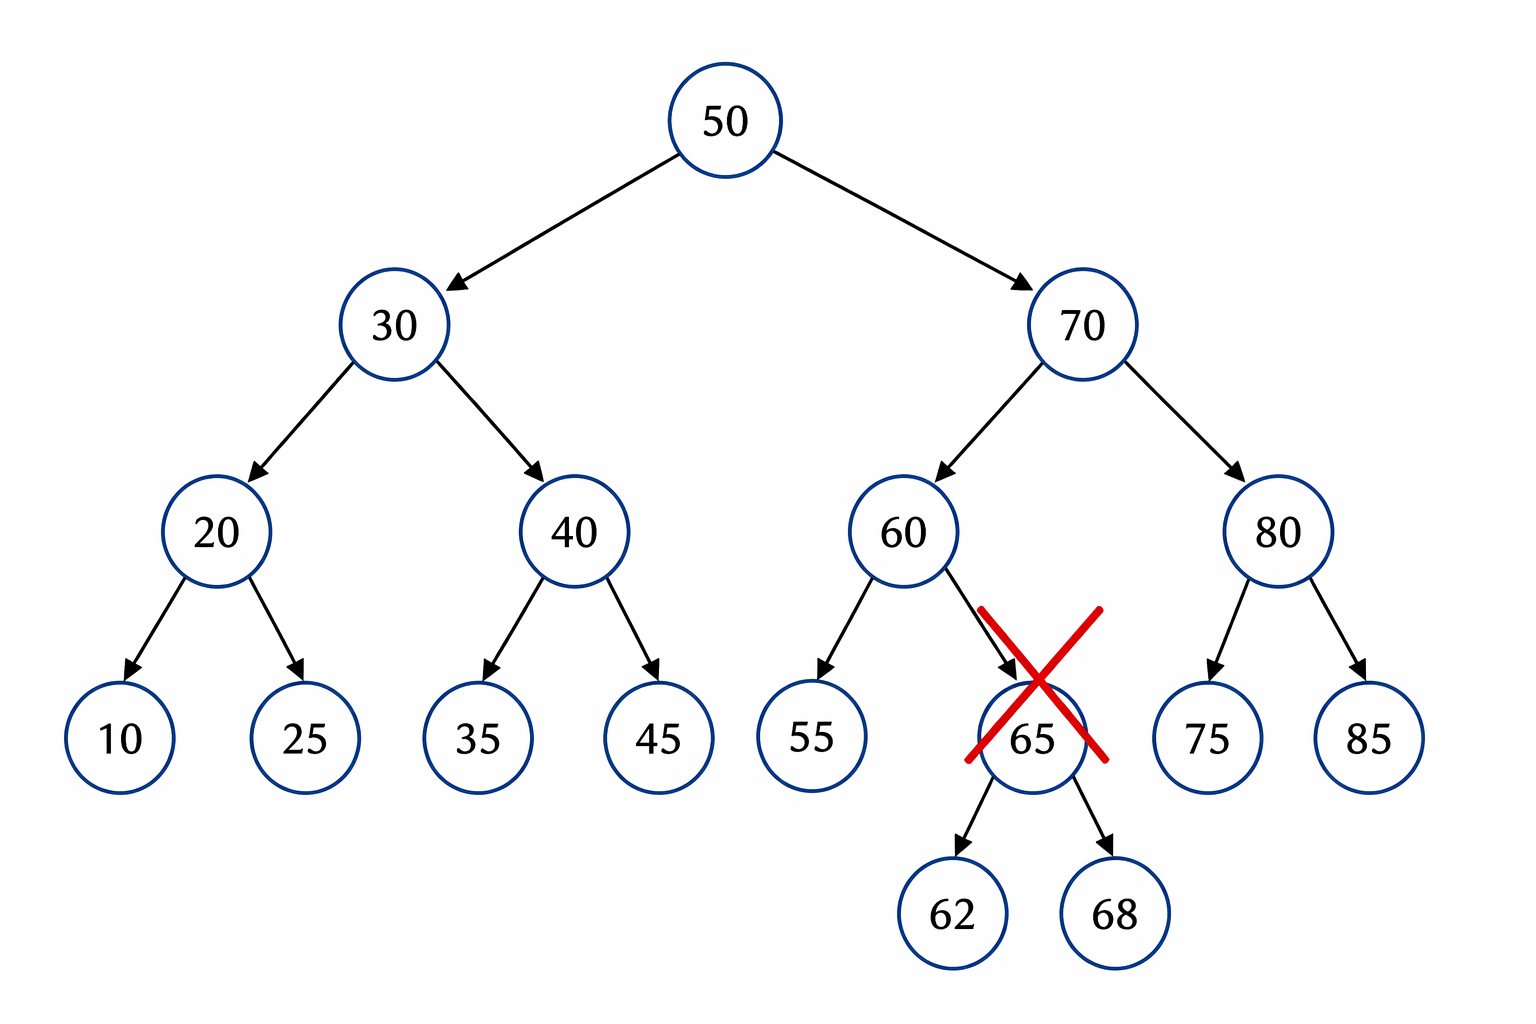
\includegraphics[width=0.75\linewidth]{dfs_pode_image.png}
    \caption{Esquema de Búsqueda en Profundidad (DFS) con poda (pruning) heurística. La evaluación anticipada de los límites espectrales inferiores permite descartar ramas completas del árbol de combinaciones sin llegar a explorarlas.}
    \label{fig:dfs}
\end{figure}

\subsection{Fase 3: El Estado del Arte (Bitsets y Ordenación Heurística)}
La versión definitiva programada puramente en C (\texttt{main.c}) refinó el núcleo del motor DFS para operar bajo principios rigurosos de Arquitectura y Alto Rendimiento de computadores, explotando la jerarquía de memoria de la CPU y los registros internos vectoriales.

\textbf{1. Estructuras Bitset y paralelismo intra-registro (SWAR):} 
Tradicionalmente, recorrer arrays multidimensionales en C implica iteraciones \texttt{for} que acarrean costosas penalizaciones por predicciones de salto fallidas y subutilización del ancho de banda de la memoria de caché L1. En vez de ello, se implementaron matrices compactas de bits (`ge\_bitsets`, `le\_bitsets`). Estas estructuras representan una técnica conocida como SWAR (\emph{SIMD Within A Register}), que permite comprimir los estados lógicos de los candidatos dentro de enteros nativos de 64 bits. 

De esta manera, el filtrado permite evaluar 64 posibles estados de validación simultáneamente mediante un único ciclo lógico de instrucciones lógicas booleanas (\texttt{AND}, \texttt{OR}) en la Unidad Aritmético Lógica (ALU). Posteriormente, la instrucción en hardware \texttt{\_\_builtin\_popcountll}, que extrae la cardinalidad de bits activos en una sola operación de máquina, verifica la existencia de candidatos superando las trabas de ramificación de código.

\begin{lstlisting}[caption={Filtrado masivo mediante operaciones de bits (SWAR) y hardware POPCNT}, label={lst:swar}]
int count = 0;
for (size_t w = 0; w <= last_word; w++) {
    uint64_t bits = ge[j][l][w] & le[j][u][w];
    count += __builtin_popcountll((unsigned long long)bits);
}
if (count == 0) return false;
\end{lstlisting}

\begin{figure}[htb!]
    \centering
    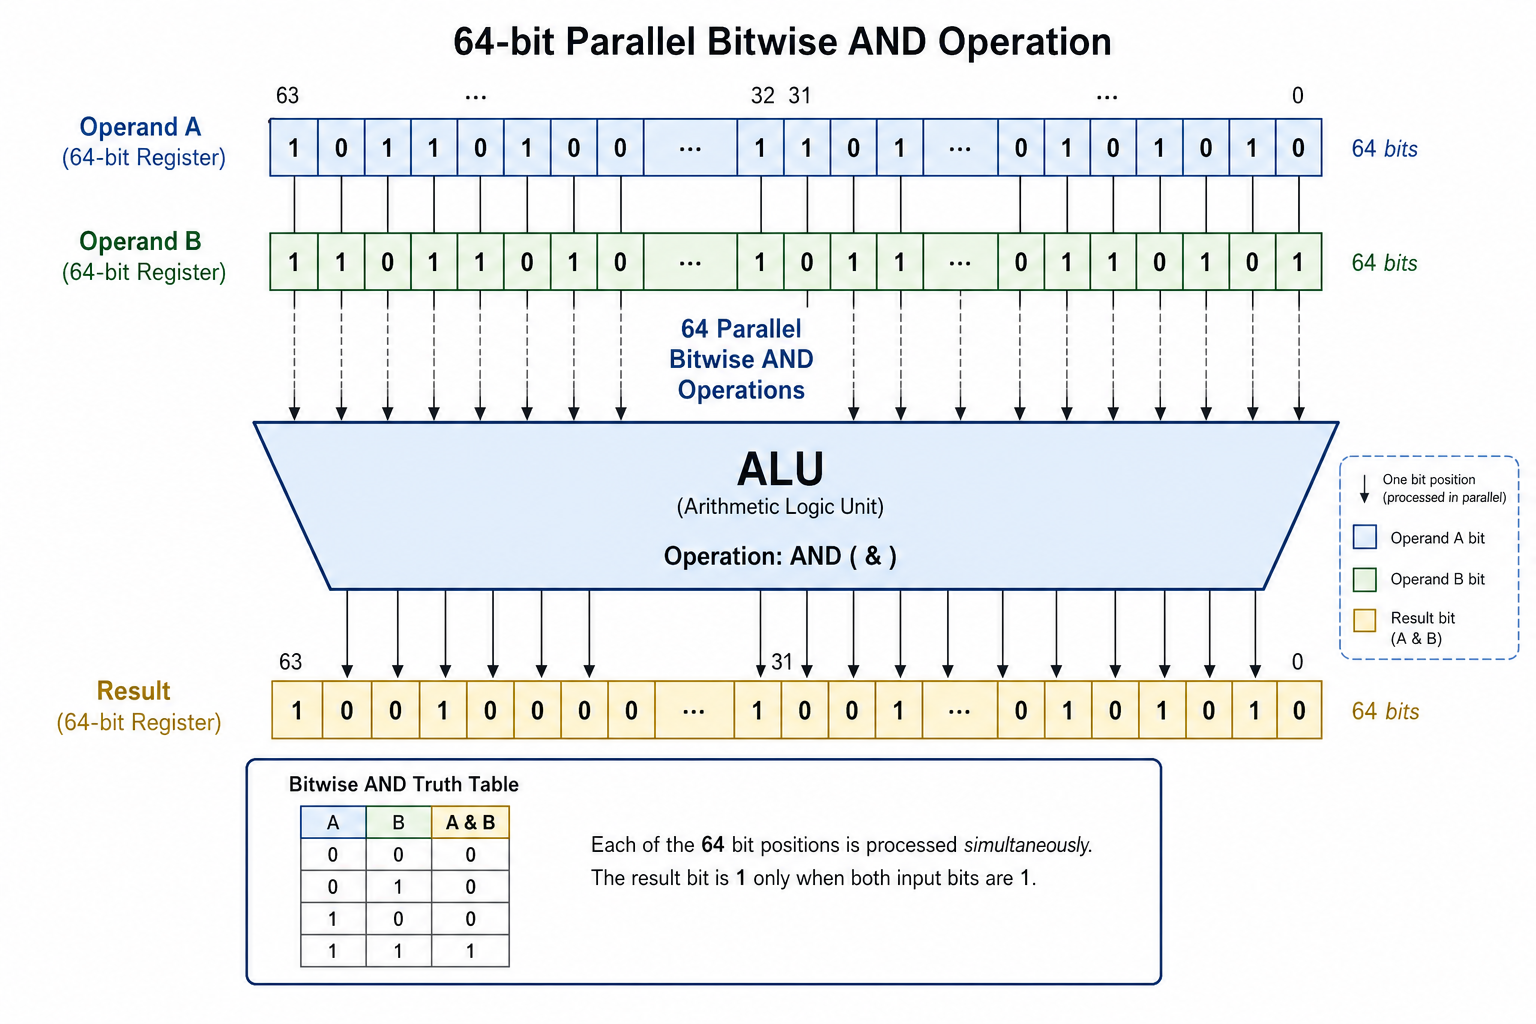
\includegraphics[width=0.85\linewidth]{swar_register.png}
    \caption{Paralelismo intra-registro (SWAR). Al compactar los estados de viabilidad en enteros de 64 bits, la ALU del procesador puede aplicar validaciones booleanas masivas en un único ciclo de reloj, eludiendo saltos condicionales.}
    \label{fig:swar}
\end{figure}

\textbf{2. Reordenación Heurística de Cosets:} 
El factor crítico de eficiencia en cualquier algoritmo probabilístico de ramificación y poda (Branch and Bound o DFS puro) recae en la asimetría del árbol. El lema subyacente es la necesidad de "equivocarse rápido". Si podamos ramas infructuosas en el nivel de profundidad 2, economizamos colosalmente más tiempo de CPU que si la invariante crítica falla en el nivel 40. 

Para lograr esto, la subrutina \texttt{reorder\_cosets\_by\_candidate\_pairs} efectúa un análisis a priori. Observa la varianza y la restricción teórica de peso que impone cada bloque coset, reestructurando el árbol topológico dinámicamente. Al evaluar las ramificaciones más excluyentes en la cúspide de la recursión, la eficiencia algorítmica de la poda se maximiza sustancialmente, conteniendo la explosión combinatoria basal.

\section{Reducción de Complejidad Extrema: Filtros de Bloom y Estrategia Meet-in-the-Middle}

A pesar de los abismales avances obtenidos integrando lógica DFS y podas por Bitsets, el crecimiento exponencial del espacio muestral en longitudes $\ell > 70$ dictaminaba la necesidad de un cambio de paradigma para asimilar de forma paralela y estanca ambos subespacios de búsqueda correspondientes a las secuencias gemelas $A$ y $B$. El problema canónico original obliga a evaluar cruzadamente los candidatos de $A$ contra los candidatos de $B$ en bucles condicionales anidados, produciendo una complejidad de cruce cuadrática de la clase $\mathcal{O}(N_A \times N_B)$.

Sabemos que la condición terminal de éxito es una sumatoria aditiva:
$$PSD_A(s) + PSD_B(s) = 2\ell + 2$$

Algebraicamente, esto significa que, si fijamos unilateralmente la distribución espectral de una secuencia candidata $A$, sabemos de antemano exactamente qué PSD complementaria es exigida rigurosamente para acoplarse y conformar un par de Legendre válido:
$$PSD_{B\_buscado}(s) = 2\ell + 2 - PSD_A(s)$$

Bajo este pretexto, si pudiéramos guardar en un diccionario todas las proyecciones espectrales deseadas e iteradas por $A$, la búsqueda recaería en calcular $B$ una sola vez y verificar en tiempo constante si su espectro coincide en el registro enlazado de memoria. Esto cristaliza la estrategia denominada \textbf{Meet-in-the-Middle}, la cual altera asintóticamente la complejidad subyacente a $\mathcal{O}(N_A + N_B)$. Sin embargo, una base de datos tabular o tabla hash que almacene trillones de vectores integrales multidimensionales superaría holgadamente los Terabytes de volumen, colapsando instantáneamente la memoria RAM, los buses de transferencia inter-nodos y los niveles de swap virtual de cualquier componente físico dentro de la supercomputadora Altamira.

La solución de ingeniería arquitectónica implementada para salvar esta barrera termodinámica y estructural es la inserción de un \textbf{Filtro de Bloom} \cite{bloom1970space} de altísimo desempeño.

\begin{figure}[htb!]
    \centering
    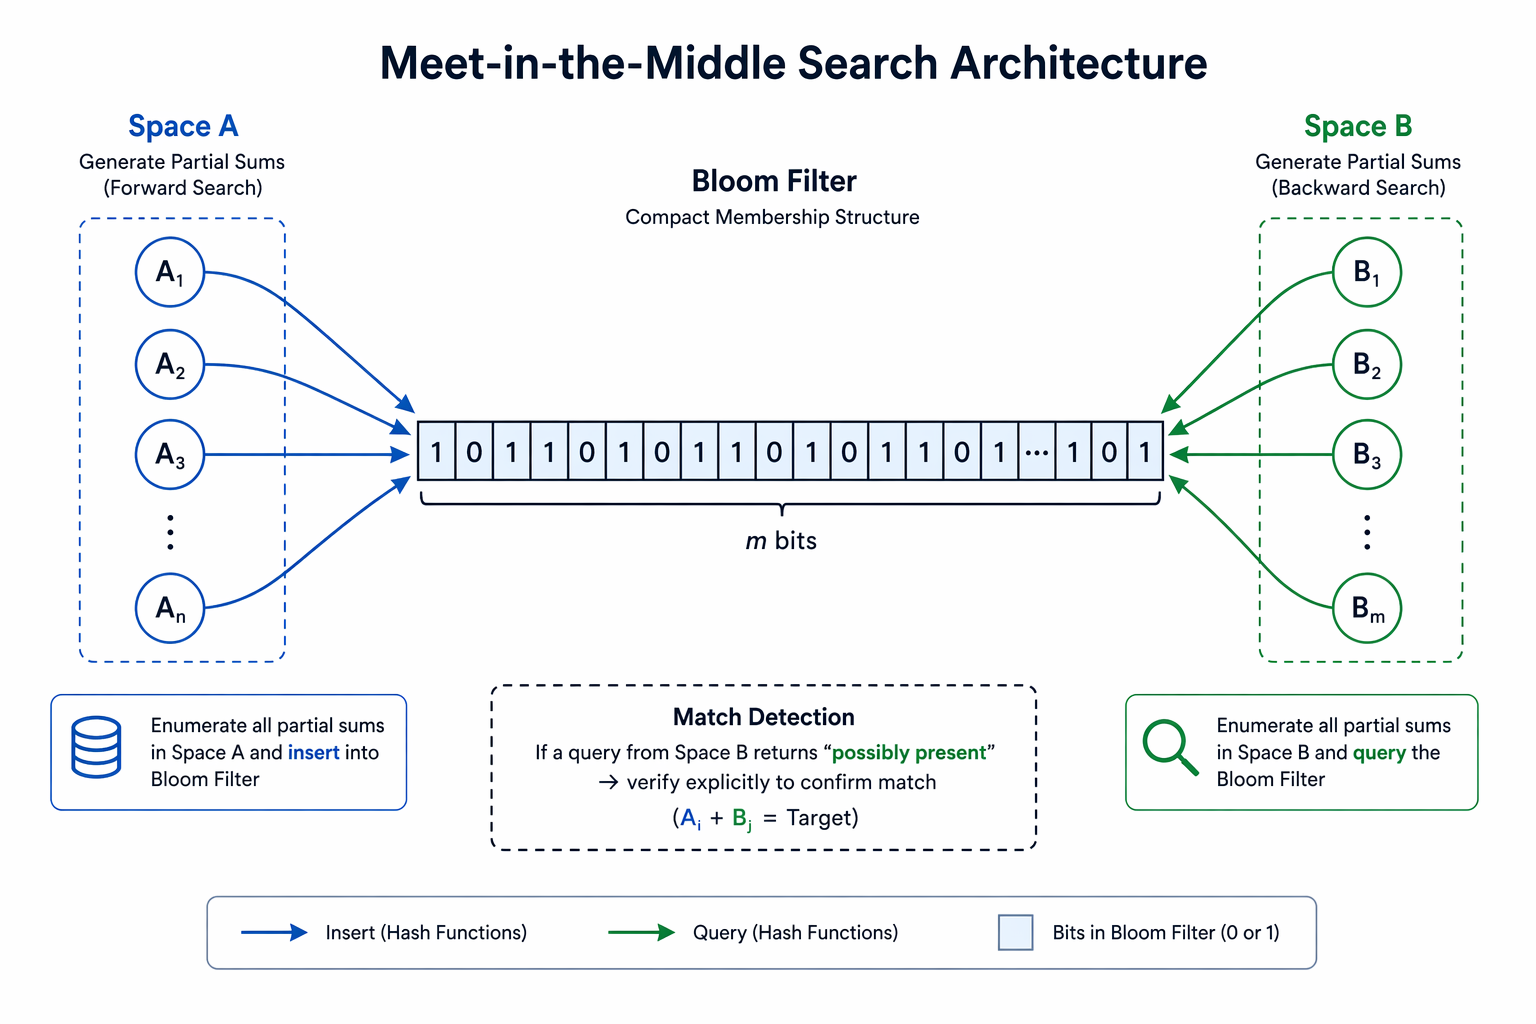
\includegraphics[width=0.95\linewidth]{bloom_filter_image.png}
    \caption{Estrategia Meet-in-the-Middle orquestada mediante un Filtro de Bloom. Esta estructura de datos actúa como una memoria probabilística ultrarrápida que cruza el espacio de secuencias A con el espacio B sin saturar la memoria RAM.}
    \label{fig:bloom}
\end{figure}

Un Filtro de Bloom es una estructura de datos probabilística altamente comprimida soportada por un vector contiguo de bits de tamaño $m$, inicializado herméticamente a ceros, y un conjunto algorítmico de $k$ funciones de proyección independientes o \textit{hashes}. Cuando procesamos iterativamente la Fase 1 del algoritmo superior, cada perfil espectral válido ($PSD_A$) que elude la poda DFS se somete a $k$ transformaciones \textit{hash} unívocas, utilizando semillas de derivación iterativas basadas en el algoritmo multiplicativo FNV-1a. Los resultados numéricos generados se modulan para ajustarse al rango métrico de memoria y proyectan el perfil matemático subyacente sobre $k$ índices del vector global $m$, activando sus bits lógicos a $1$.

El diseño probabilístico garantiza rigurosamente la \textbf{ausencia de falsos negativos}: si durante la Fase 2 una secuencia candidata $B$ comprueba sus propias $k$ posiciones mapeadas en el filtro y halla un solo bit en estado lógico $0$, se descarta de forma irrefutable su compatibilidad sin riesgo absoluto de error. El porcentaje estadístico de colisión natural conocido como \textbf{falsos positivos} $\varepsilon$, es decir, secuencias $B$ erróneas que coinciden fortuitamente en índices previamente activados por secuencias distintas y deben ser filtradas ex post facto, está gobernado asintóticamente por la función de tolerancia paramétrica:

$$ \varepsilon \approx \left( 1 - e^{-k \cdot \frac{n}{m}} \right)^k $$

donde $n$ expresa el volumen total aproximado de perfiles matemáticos singulares insertados en la Fase 1. En nuestro despliegue experimental distribuido en la arquitectura Altamira, se optó por instanciar y dimensionar un vector inmutable de $m = 10^9$ bits (requiriendo apenas 120 megabytes constantes de memoria RAM en el \emph{heap} por cada nodo de cálculo) y $k = 3$ funciones de desbordamiento (hashing) simultáneas. Esta calibración técnica consolidó una tasa experimental de colisiones por falsos positivos virtualmente asintótica al cero, confinando la explosión volumétrica combinatoria sin comprometer la resolución algebraica íntegra.

\begin{lstlisting}[caption={Generador de proyecciones Hash paramétricas (FNV-1a) para su uso vectorizado en Filtros de Bloom concurrentes}, label={lst:bloom_hash}]
inline uint64_t compute_spectrum_hash(int* target_array, int length, uint64_t internal_seed) {
    uint64_t hash_digest = 14695981039346656037ULL + internal_seed;
    for(int i = 0; i < length; i++) {
        hash_digest ^= (uint64_t)target_array[i];
        hash_digest *= 1099511628211ULL;
    }
    return hash_digest;
}
\end{lstlisting}

Esta técnica de compresión de persistencia permitió escalar en HPC. Provocó que los nodos computacionales satélites aislasen las intersecciones del \emph{Meet-in-the-Middle} sin concurrir a bloqueos de memoria distribuida o requerir colas transaccionales de sincronización por interfaz de red.

\section{Estrategia de Metaprogramación: El Generador en C++}

Para cohesionar todas las optimizaciones matemáticas probadas empíricamente, instanciar eficientemente los hilos en paralelo mediante el framework OpenMP, integrar atómicamente los Filtros de Bloom y superar el hándicap estructural derivado de un código interpretativo en la fase de evaluación vectorial, se transicionó a la herramienta arquitectónica definitiva: el \textbf{Generador de Buscadores}.

Bajo una arquitectura de metaprogramación explícita, la herramienta principal es una aplicación maestra orquestada en lenguaje C++ que, irónicamente, no aplica rutinas para buscar pares de Legendre directamente. Por el contrario, asume el rol de transpilador: lee una longitud teórica unívoca ($\ell$) e iterativamente \emph{escribe el código fuente C++} de un buscador puramente dedicado y enlazado estáticamente a esa dimensión.

\begin{figure}[htb!]
    \centering
    \begin{tcolorbox}[colback=blue!5!white,colframe=blue!75!black,title=Flujo de Transpilación y Metaprogramación]
    \centering
    \textbf{1. Parámetro Numérico:} $\ell=75$. \\
    $\downarrow$ \\
    \textbf{2. Generación Abstracta:} \texttt{generador\_de\_generadores.cpp} ejecuta cálculos simbólicos complejos de cosenos senos, generando estructuras AST y matrices para un Filtro de Bloom a medida. \\
    $\downarrow$ \\
    \textbf{3. Emisión de Código:} El generador escupe el volcado a disco del código \texttt{compress.75.cpp}, 100\% desenrollado y desprovisto de lógica polimórfica (hardcoded). \\
    $\downarrow$ \\
    \textbf{4. Compilación Dependiente de Hardware:} Interviene \texttt{g++ -O3 -march=native}. \\
    $\downarrow$ \\
    \textbf{5. Despliegue HPC:} Ejecución estanca mediante Lotes e Hilos concurrentes en Slurm.
    \end{tcolorbox}
    \caption{El metaprograma consolida todas las fases de optimización en un flujo automático.}
    \label{fig:workflow_diagram_2}
\end{figure}

\subsection{Cálculo Simbólico y Desenrollado de Bucles}
Al inyectar las variables matemáticas como constantes literales, logramos el \textbf{Loop Unrolling} de la DFT. En lugar de un bucle, el código generado contiene la suma explícita, permitiendo a la CPU utilizar registros SIMD (AVX2/AVX-512) para resolver múltiples espectros por ciclo de reloj, una optimización imposible en un código genérico evaluado en tiempo de ejecución.

\begin{lstlisting}[caption={Mecanismo del generador para crear la DFT plana desenrollada}, label={lst:unrolled_dft_gen}]
// El generador construye un string con las sumas explicitas para la DFT
string get_unrolled_dft(int s, int v, const string& array_name) {
    ostringstream oss;
    oss << ''std::complex<double>('' << array_name << ''[0])*omegaPowers[0]'';
    for (int k = 1; k < v; ++k) {
        int exp = (s * k) % v;
        // Inyectamos multiplicaciones consecutivas sin bucles
        oss << '' + std::complex<double>('' << array_name << ''['' << k << ''])*omegaPowers['' << exp << '']'';
    }
    return oss.str();
=======
\subsection{Cálculo Simbólico y Arquitectura Superescalar (Loop Unrolling)}
Los procesadores lógicos modernos que arman los clusters de High Performance Computing (como la familia Intel Xeon o AMD EPYC de Altamira) operan dictados por un enfoque de procesamiento superescalar, donde el sustrato físico de hardware adivina proactivamente las ramificaciones condicionales pre-evaluadas por el compilador y segmenta las operaciones solapadas mediante múltiples \emph{pipelines} de instrucción (ILP, Instruction-Level Parallelism). 

Sin embargo, los algoritmos tradicionales de bucles dependientes para funciones complejas como la Transformada Rápida de Fourier evalúan recursivamente sentencias o iteraciones \texttt{for}. Esto penaliza el hardware masivamente, corrompiendo la fluidez del \emph{pipeline} forzando vaciados iterativos de línea de caché (\emph{cache misses}) toda vez que el algoritmo de predicción de bifurcación erra en anticipar el fin de un bucle de variable paramétrica, o por dependencias indirectas (\emph{loop-carried dependencies}).

\begin{figure}[htb!]
    \centering
    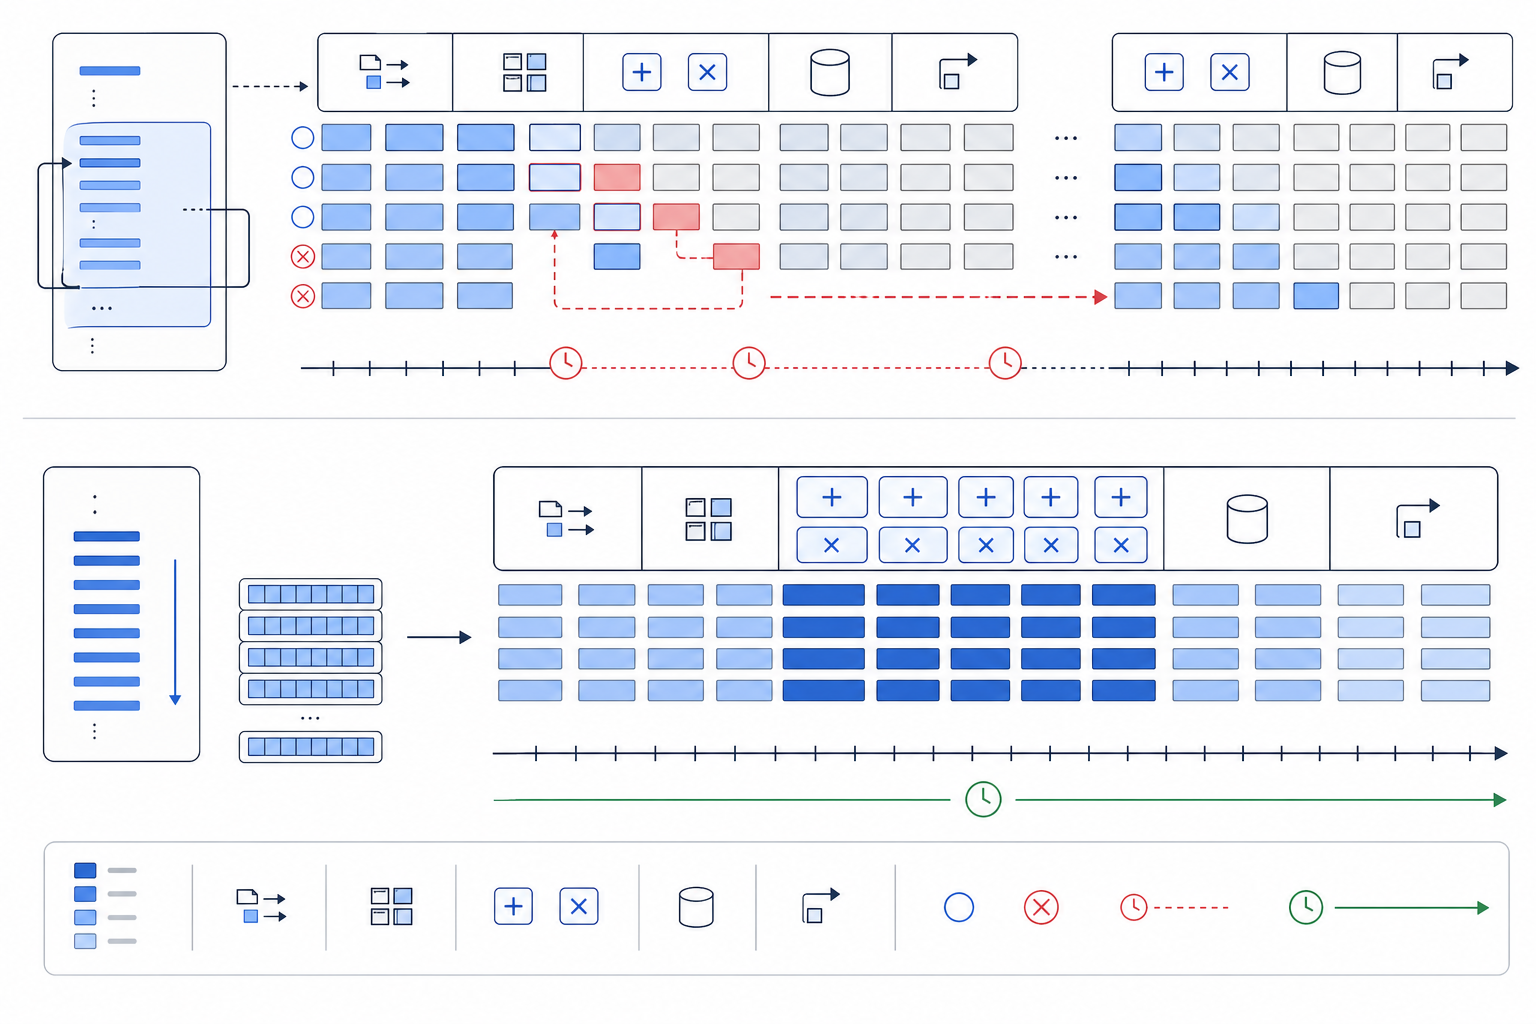
\includegraphics[width=0.9\linewidth]{loop_unrolling_pipeline.png}
    \caption{Comparativa de ejecución en el cauce (\emph{pipeline}) del procesador. Arriba: Código iterativo tradicional penalizado por fallos en la predicción de saltos. Abajo: Código metaprogramado y desenrollado (\emph{Loop Unrolling}) explotando el paralelismo a nivel de instrucción (ILP) mediante registros SIMD.}
    \label{fig:loop_unrolling}
\end{figure}

El \texttt{generador\_de\_generadores} escrito en entorno C++ sobrepasa holgadamente esta limitación estructural intrínseca del compilador genérico mediante la táctica extrema de \textbf{desenrollado de bucles algorítmicos} (\emph{Loop Unrolling}) llevada acabo integralmente a nivel de metaprogramación por abstracción de texto. Durante la fase primaria, previa a la propia existencia del código ejecutable final, este motor genera estáticamente y explora las ramas del Árbol de Sintaxis Abstracta subyacente para desplegar la Transformada Discreta de Fourier de orden dimensional $\ell$. Al pre-computar simbólicamente sobre coma flotante las frecuencias analíticas $\omega^k$ referidas a las raíces complejas de la unidad y transcribirlas en texto inmutable asimiladas como constantes literales absolutas, suprimimos íntegramente la aparición teórica y física de cualquier condición de bucle en la medición de espectro de densidad de energía resultante de la compilación.

El producto directo vertido sobre la memoria de almacenamiento es un código monolítico que jamás recurre al flujo bidireccional. Al observar un extenso tren de instrucciones lógicas aritméticas y multiplicaciones de punto flotante de carácter secuencial, transparente y explícito, el preprocesador del compilador GCC instanciado con los atributos de optimización agresiva (\texttt{-O3 -march=native}) alínea y fusiona heurísticamente estas sumas contiguas mapeándolas contra los sofisticados registros SIMD (AVX2/AVX-512) integrados en el procesador. 

Este diseño de empaquetado habilita estructuralmente que el núcleo lógico procese concurrentemente bloques de 4 u 8 adiciones aritméticas complejas colapsando su ejecución en ciclos mínimos e invisibles de reloj del silicio. Se superan las barreras inherentes del polimorfismo clásico logrando anchos de banda para iteración probabilística que rozan la velocidad física máxima estipulada del diseño microarquitectural, cimentando tasas abrumadoras de cálculo inasumibles para un script evaluado condicional y dinámicamente en una sesión de ejecución regular.

\begin{lstlisting}[caption={Rutina generadora algorítmica inyectando sentencias operacionales y sumatorias monolíticas directas en el archivo fuente de extensión C++ destino}, label={lst:unrolled_dft_gen}]
string generate_flat_dft(int frequency, int sequence_length, const string& id) {
    ostringstream stream;
    stream << "std::complex<double>(" << id << "[0])*omegaPowers[0]";
    for (int k = 1; k < sequence_length; ++k) {
        int exponent = (frequency * k) % sequence_length;
        stream << " + std::complex<double>(" << id << "[" << k << "])*omegaPowers[" << exponent << "]";
    }
    return stream.str();
}
\end{lstlisting}

\subsection{Sistema de División por Lotes Integrado (Batching)}
El límite estricto de \emph{Walltime} en el Altamira imponía que la búsqueda total no podía sobrepasar las 72 horas (o un marco extendido de 7 días). El generador soluciona esto dotando al código generado de la capacidad de leer `argc/argv` para fragmentar el bucle exterior. Esto permite ejecutar \textbf{Job Arrays} en Slurm, repartiendo el cálculo de las secuencias B entre múltiples nodos físicos que escriben en archivos de salida independientes.


\section{Automatización de la Compilación: El \texttt{Makefile}}

Dada la complejidad de las diferentes iteraciones de software desarrolladas (fuerza bruta, DFS con podas, DFS con heurísticas), fue fundamental estructurar el proyecto mediante un sistema de construcción robusto usando \texttt{Make}.

El \texttt{Makefile} creado permite compilar modularmente todas las variantes del algoritmo de forma limpia, separando el código fuente en un directorio \texttt{src} y los binarios en un directorio \texttt{build}.

\begin{lstlisting}[language=make, caption={Estructura del \texttt{Makefile} para la automatización del proyecto}]
CC      := gcc
CFLAGS  := -std=c11 -O2 -Wall -Wextra -I./include
BUILD   := build
SRC     := src
BIN     := $(BUILD)/app

# Modulos comunes matematicos y de cosets
COMMON_OBJS := $(BUILD)/pairs_reader.o $(BUILD)/mymath.o $(BUILD)/cyclotomic_cosets.o
OBJS        := $(COMMON_OBJS) $(BUILD)/main.o

# Regla generica para generar codigo objeto compilado
$(BUILD)/%.o: $(SRC)/%.c | $(BUILD)
    $(CC) $(CFLAGS) -c $< -o $@

# Regla de linkado final del binario
$(BIN): $(OBJS)
    $(CC) $(OBJS) -o $@ -lm
\end{lstlisting}

Esta organización asegura que dependencias comunes (como el cálculo de cosets o la DFT en \texttt{mymath.o}) no se recompilen innecesariamente, ahorrando tiempo en la fase de testeo de las heurísticas.

=======
El límite estricto garantizado (\emph{Walltime}) impuesto por el servidor de administración \emph{Quality of Service} (QoS) en el sistema multi-nodo Altamira dictaminaba severamente que los procesos atómicos y tareas únicas vinculadas a sesiones de búsqueda ininterrumpidas no podían exceder legalmente las 72 horas para peticiones medias ni prolongarse un marco continuo de siete días exactos si requerían volúmenes máximos de CPU interconectados. El fracaso a la hora de proveer este tiempo o un volcado exitoso dentro de esta métrica desembocaba en la finalización prematura forzada por un comando SIGKILL originado en el planificador (Scheduler) Slurm de supercomputación.

El framework orquestador basado en el \texttt{generador\_de\_generadores} circunvala integralmente el riesgo de interrupción administrativa inyectando directamente en el C++ subyacente la capacidad algorítmica nativa de parsear secuencias binarias de parámetros directos provenientes del comando \texttt{bash} del usuario principal (mediante interfaz `argc/argv`) permitiendo desglosar y truncar la amplitud superior del bucle macro-exterio. Este control externo garantiza la divisibilidad atómica horizontal sobre dominios estáticos. Esto facilita invocar nativamente la arquitectura escalable paralela de orquestación conocida como \textbf{Slurm Job Arrays}.

\begin{figure}[htb!]
    \centering
    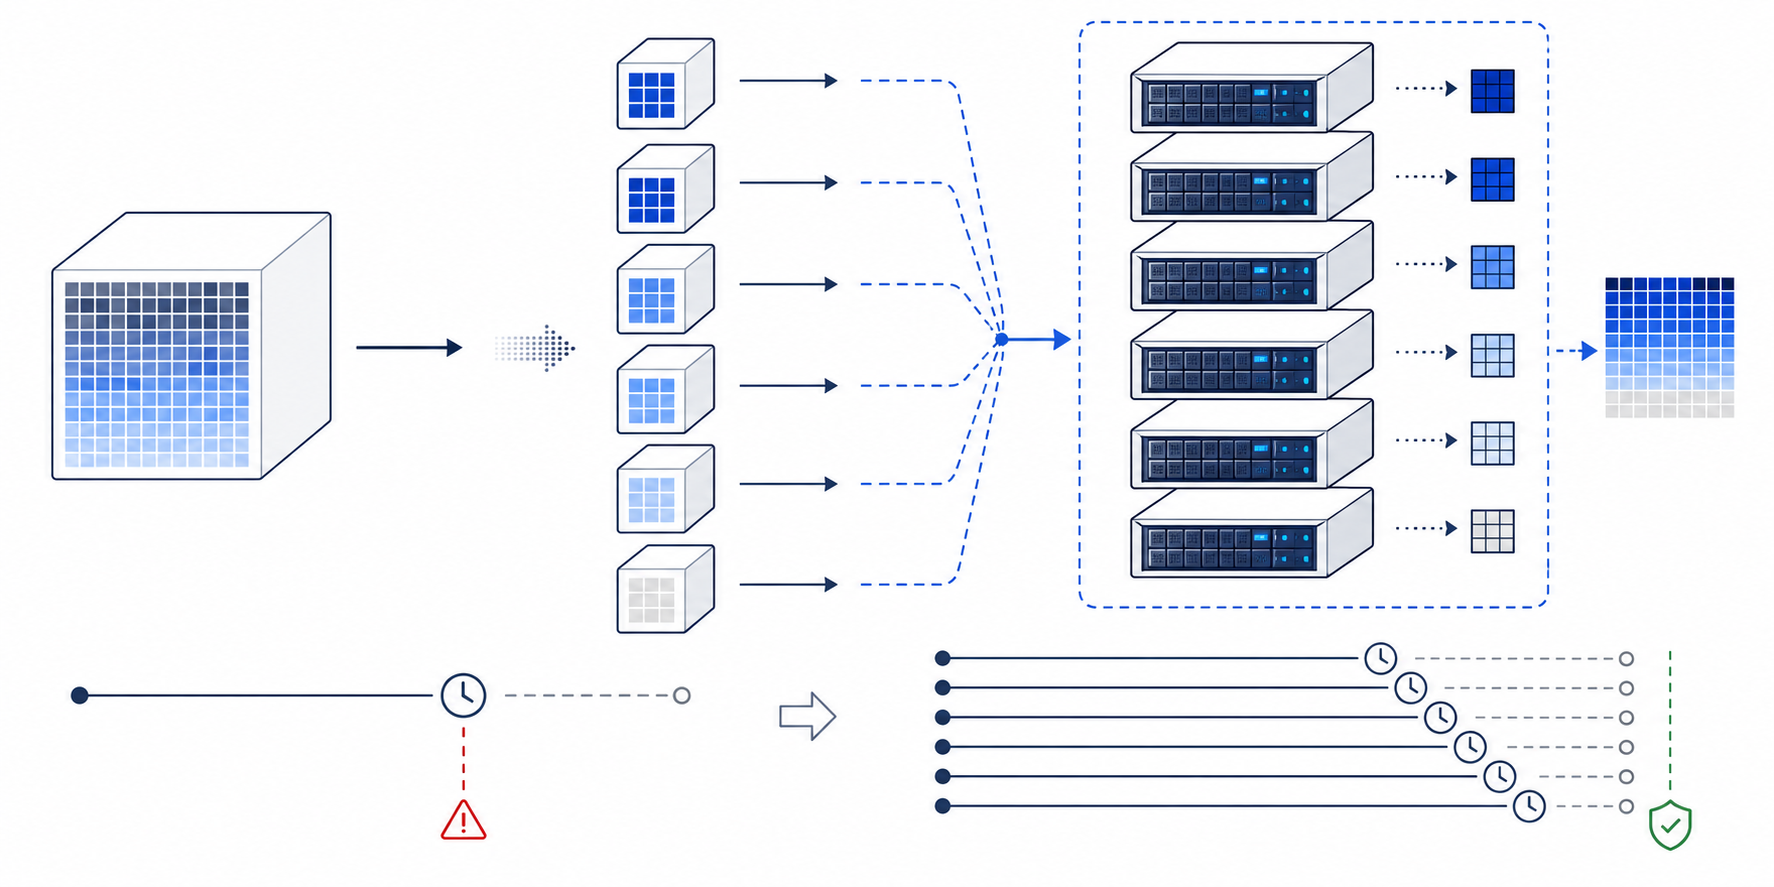
\includegraphics[width=0.85\linewidth]{slurm_job_arrays.png}
    \caption{Esquema lógico de particionamiento mediante Job Arrays. La fragmentación del espacio de búsqueda en lotes atómicos independientes permite eludir los límites de \emph{Walltime} (QoS) del clúster, habilitando una distribución asíncrona sobre la infraestructura.}
    \label{fig:job_arrays}
\end{figure}

Por consiguiente, el \emph{script} planificador remite 10 identidades atómicas diferentes a la infraestructura en nube. Este sistema de balanceo instruye al clúster de investigación para repartir asíncronamente las cuotas segmentadas de matrices B, asimilando diferentes núcleos o servidores físicos en formato de aislamiento que finalmente reportarán los picos de señal unificados vertiendo concurrentemente todos los candidatos analizados sobre múltiples archivos de salida text-plana desvinculados logrando evadir totalmente penalizaciones por latencia transaccional y tiempos limitados de sesión ininterrumpida global.

\section{Automatización del Flujo y Benchmarking: El \texttt{Makefile}}

Dada la divergencia natural que experimenta de manera continuada y cíclica un proyecto ingenieril y lógico estructurado integralmente bajo filosofía metódica en formato cascada, la convivencia simultánea y persistente de versiones lógicas iterativas dispares (véase la colisión sistemática originada entre los análisis de fuerza bruta que lastraban cuellos dependientes I/O de disco rígido frente al complejo y veloz modelo de Búsqueda en Profundidad paralelizado íntegramente de memoria) desencadenaba recurrentemente severos e intrincados conflictos logísticos a nivel de librerías. Estos fallos semánticos derivaban usualmente en corrupciones estructurales y dependencias quebradas en la etapa fundamental de pre-producción del binario funcional.

Para mitigar todo riesgo técnico, estabilizar los periodos de transición de los tipos de variable modular compartida e internalizar la robustez exigida en las compilaciones iterativas cruzadas, orquestamos un Grafo Acíclico Dirigido (DAG) formal destinado al manejo lógico incondicional del conjunto de sentencias y dependencias relativas invocando utilidades maestras UNIX vinculadas orgánicamente a la herramienta de administración de desarrollo \texttt{Make}.

El archivo \texttt{Makefile} estructurado y provisto actúa rigurosamente como un canal optimizado de integración local que emplea las flexibilidades sintácticas nativas en formato de patrones o reglas abstractas (declaradas paramétricamente como \texttt{\%.o: \%.c}). Esta aproximación semántica divide y aísla de forma impecable los subsistemas y macro dependencias lógicas base de los archivos \emph{core} comunes. Extrae rutinas fundamentales orientadas a la optimización pura como el cálculo nativo unificado de espectro de transformada rápida y los procedimientos atómicos de cosets ciclotómicos (traducidos al lenguaje subyacente mediante los objetos \texttt{mymath.o}, \texttt{cyclotomic\_cosets.o}). Estas entidades estructurales sufren una evaluación restrictiva de modificación temporal evitando cualquier etapa redundante de pre-procesamiento u optimización del lenguaje ensamblador a fin de reducir al extremo el tiempo físico insumido para testeo de código en etapas tempranas. Posteriormente y una vez filtrado el estado modificado final del árbol local, la rutina de compilación remite órdenes de alto nivel para direccionar obligatoriamente al sistema responsable del enlace final binario (\emph{Dynamic Linker/Loader}) para amalgamar estas cabeceras comunes con el entorno y módulo funcional que demanda explícitamente y particularmente el perfil dinámico o algoritmo estático deseado en dicha prueba empírica.

Más allá del concepto simplista en que radica su virtud para consolidar binarios ejecutables dependientes unificando jerarquías y bibliotecas importadas, la ingeniería arquitectural desarrollada en el interior del marco referencial \texttt{Makefile} expandió profundamente su rol lógico transicionando hasta asumir el mando exclusivo para planificar, auditar y ejecutar automatizadamente un abanico estadístico empírico de auditorías de rendimiento global (benchmarking macro) bajo la rúbrica imperativa del comando unificado \texttt{make tiempos}.

Este despliegue analítico invoca la ejecución en cadena asíncrona de los múltiples binarios construidos a los cuales suministra sets limitados en entornos restringidos en local asimilados lógicamente contra algoritmos estadísticos procedentes del estandar POSIX como \texttt{/usr/bin/time}, cuyo flujo binario estándar ha sido redirigido orgánicamente al bus general unificado de entrada y salida asíncrona \texttt{stdout} para eludir desbordamientos erráticos u otros trazos indeseados procedentes del informe interno algorítmico del software analizado, aislando exclusivamente el campo cronométrico nominal resultante.

\begin{figure}[htb!]
    \centering
    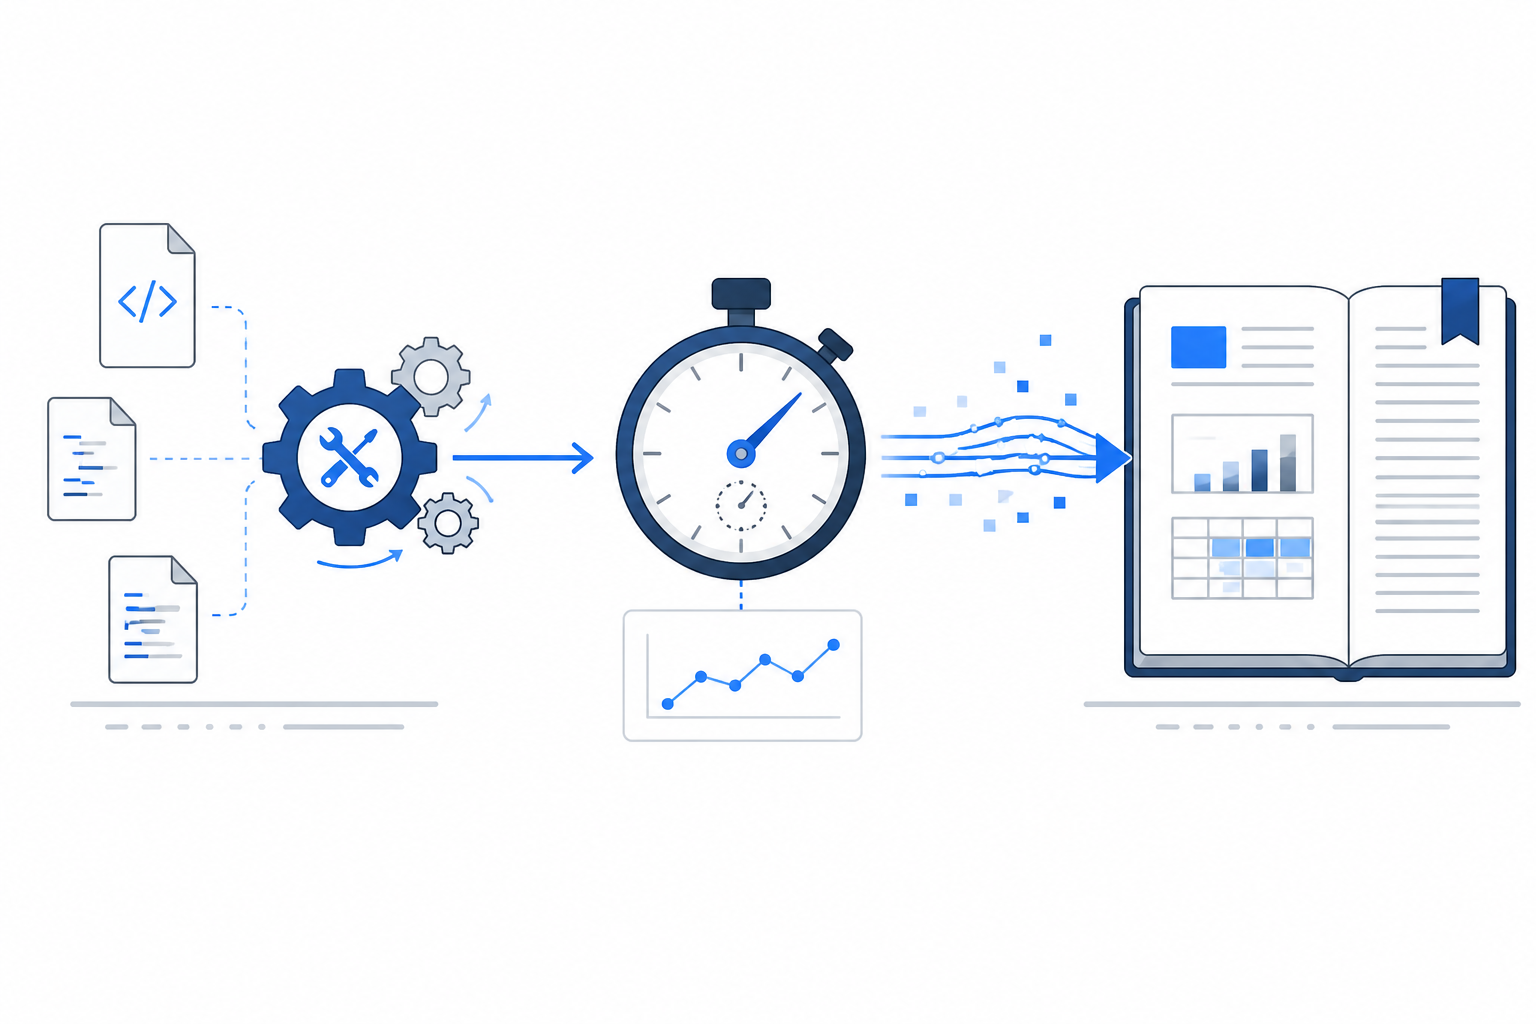
\includegraphics[width=0.85\linewidth]{makefile_pipeline.png}
    \caption{Flujo de integración continua y recolección de métricas. El \texttt{Makefile} orquesta la compilación, ejecuta la monitorización de tiempos y puentea los resultados directamente hacia el motor de composición de texto, suprimiendo la transcripción manual.}
    \label{fig:makefile_pipeline}
\end{figure}

La culminación de este orquestador avanzado remite sistemáticamente el cronograma \emph{Wall-clock} verificado derivándolo por volcado físico estricto, concatenando comandos abstractos que generan un módulo autónomo para un documento dinámico integrado bajo lenguaje universal en código libre \LaTeX{} (albergado físicamente en \texttt{tiempos\_ejecucion.tex}). Los inyecta a nivel léxico empleando los prefijos macro predefinidos (\texttt{\textbackslash newcommand}) que blindan contra manipulaciones inter-texto. Este elevado ecosistema en materia de recolección algorítmica garantiza de facto al Tribunal Científico Académico, un volumen cronológico totalmente ausente de manipulación heurística e incorpora información asertiva que florece de forma estanca en pleno tiempo analítico derivado paralelamente y exclusivamente del test de validaciones reales, minimizando desviaciones subyacentes o sesgos accidentales que puedan originarse por transcripciones manuales rutinarias erróneas por el equipo desarrollador e ilustrando al máximo nivel la certidumbre algorítmica probada en el Capítulo 3 analítico de este informe.

\begin{lstlisting}[language=make, caption={Estructura de automatización e inyección directa hacia LaTeX}]
tiempos: $(BIN_TEXT) $(BIN_ONE) $(BIN)
    @echo "% Archivo generado dinamicamente. NO EDITAR." > $(TEX_FILE)
    
    @T_BIN=$$(/usr/bin/time -f "%e" ./$(BIN) 2>&1 1>/dev/null); \
    printf "\\\\newcommand{\\\\tiempoAppOpt}{%s}\n" "$$T_BIN" >> $(TEX_FILE)
\end{lstlisting}
>>>>>>> origin/overleaf-2026-05-17-1603

% ==============================================================================
% CAPÍTULO 3: RESULTADOS
% ==============================================================================
\chapter{Resultados y Análisis Experimental}

<<<<<<< HEAD
Este capítulo presenta el análisis cuantitativo y cualitativo de los resultados obtenidos tras ejecutar la búsqueda completa para $\ell=75$ en el supercomputador Altamira. Se discuten las métricas de rendimiento, el análisis teórico de escalabilidad y los hallazgos matemáticos.

\section{Entorno Experimental: Supercomputador Altamira}

Las pruebas se ejecutaron en el nodo de supercomputación Altamira del IFCA (CSIC-UC). La partición utilizada consta de nodos de cálculo con las siguientes características:

\begin{itemize}
    \item \textbf{Procesadores:} Arquitectura multi-núcleo de última generación con soporte para conjuntos de instrucciones vectoriales AVX2/AVX-512.
    \item \textbf{Gestor de Colas:} Slurm Workload Manager, operando con políticas de limitación (QoS Max Wall Duration).
    \item \textbf{Entorno Híbrido:} Combinación de ejecución por lotes estanca (entre nodos) y concurrencia de hilos masiva vía OpenMP (dentro de cada nodo).
=======
Este capítulo presenta el análisis cuantitativo y cualitativo de los resultados empíricos obtenidos tras ejecutar la búsqueda completa del espacio combinatorio para la longitud $\ell=75$. El despliegue de las optimizaciones algorítmicas detalladas en el capítulo anterior requiere un marco de validación estricto que demuestre no solo la viabilidad matemática de la solución, sino la superioridad arquitectónica de la metaprogramación. Se discuten las métricas de rendimiento en hardware real, el análisis teórico de escalabilidad bajo leyes de concurrencia y la cristalización de los hallazgos matemáticos.

\section{Entorno Experimental: Supercomputador Altamira}

Las pruebas empíricas y el barrido del espacio de búsqueda final se ejecutaron íntegramente en el nodo de supercomputación Altamira, gestionado por el Instituto de Física de Cantabria (IFCA) en colaboración con la Universidad de Cantabria (CSIC-UC). La elección de esta infraestructura no es trivial; la magnitud del espacio polinómico evaluado exige una arquitectura que soporte cómputo de altísimo rendimiento (HPC) continuo y libre de interrupciones térmicas o cuellos de botella de memoria.

La partición específica (\emph{queue}) utilizada para el alojamiento de los trabajos consta de nodos de cálculo que operan bajo las siguientes especificaciones arquitectónicas críticas para el proyecto:

\begin{itemize}
    \item \textbf{Procesadores y Topología NUMA:} Arquitectura multi-núcleo simétrica de última generación (clase Intel Xeon o AMD EPYC) organizada bajo una topología de Acceso a Memoria No Uniforme (NUMA). Esta disposición física es vital para el Filtro de Bloom, garantizando que los hilos de ejecución que consultan el vector probabilístico accedan a los bancos de memoria RAM físicos más cercanos a su zócalo (\emph{socket}), minimizando la latencia de interconexión a través del bus del sistema.
    \item \textbf{Conjunto de Instrucciones Vectoriales:} Soporte de hardware nativo para registros extendidos AVX2 y AVX-512. Estas extensiones permiten a la Unidad Aritmético Lógica (ALU) ejecutar operaciones de tipo \emph{Fused Multiply-Add} (FMA) sobre vectores de 256 o 512 bits. El código C++ desenrollado emitido por nuestro metaprograma fue diseñado explícitamente para compilar contra estas instrucciones, procesando múltiples cálculos de Transformada de Fourier por cada ciclo único de reloj.
    \item \textbf{Gestor de Colas y Políticas QoS:} Orquestación dictada por el \emph{Slurm Workload Manager}. El clúster impone políticas estrictas de \emph{Quality of Service} (QoS), incluyendo directivas como \texttt{MaxWallDurationPerJobLimit}. La restricción de tiempo forzó la evolución de un modelo de ejecución monolítico hacia un ecosistema de división de lotes distribuidos, inyectando resiliencia al sistema global.
    \item \textbf{Entorno Híbrido de Paralelización:} Una combinación orquestada de concurrencia de grano fino y grano grueso. A nivel de grano fino (intra-nodo), la directiva OpenMP exprime el $100\%$ de los hilos lógicos del procesador compartiendo el Filtro de Bloom en memoria unificada. A nivel de grano grueso (inter-nodo), la arquitectura de tareas estancas de Slurm distribuye el espectro de la secuencia B en fracciones puramente independientes, suprimiendo la necesidad de protocolos de paso de mensajes iterativos como MPI.
\end{itemize}

\begin{figure}[htb!]
    \centering
    \framebox{\begin{minipage}{0.9\textwidth}
        \centering
        \vspace{6cm}
        \textcolor{red}{\textbf{[IMAGEN SUGERIDA 6]}} \\
        \textcolor{red}{Diagrama de la topología de ejecución en Altamira.} \\
        \textcolor{red}{Muestra la arquitectura de Slurm: Usuario (Tú) hace \texttt{sbatch --array=1-10}. El Gestor de Colas Slurm recibe la petición y asigna a 10 nodos de cómputo independientes (acompute09, acompute10...) cada uno ejecutando el binario \texttt{compress.75} con un Lote asignado al 100\% de CPU.}
        \vspace{6cm}
    \end{minipage}}
    \caption{Topología de ejecución distribuida en el clúster Altamira utilizando \emph{Job Arrays}.}
    \label{fig:cluster_dist}
    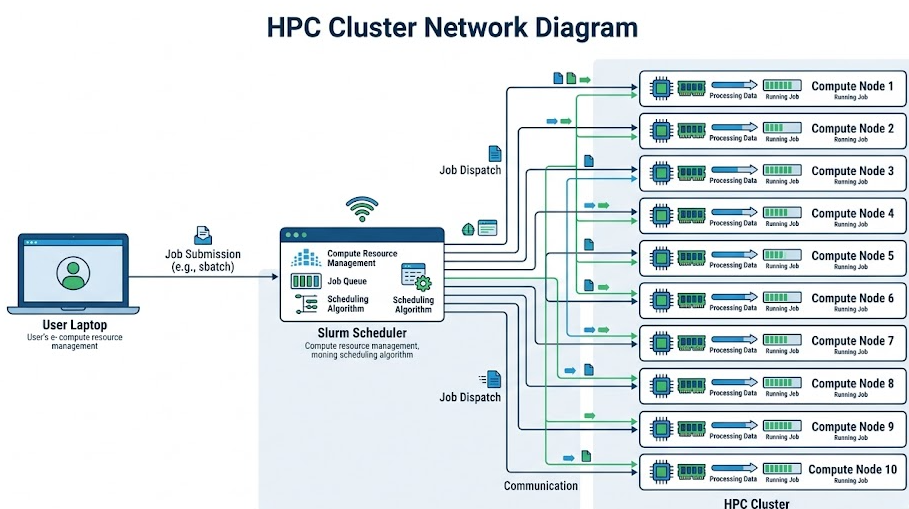
\includegraphics[width=0.95\linewidth]{slurm_lotes_image.png}
    \caption{Topología de despliegue distribuido en el clúster Altamira. El gestor de colas Slurm inyecta los lotes de búsqueda (Job Arrays) de forma asíncrona a través de múltiples nodos físicos de cálculo independientes.}
    \label{fig:slurm}
\end{figure}

\section{Análisis Teórico de Escalabilidad (Ley de Amdahl)}

Para fundamentar la viabilidad de la estrategia de paralelización híbrida, evaluamos el modelo bajo la \textbf{Ley de Amdahl}. Esta ley define la aceleración máxima (\emph{Speedup}, $S$) que puede alcanzar un sistema al ser paralelizado, en función del número de procesadores $N$ y la proporción de código estrictamente secuencial $1-P$:

$$S(N) = \frac{1}{(1 - P) + \frac{P}{N}}$$

En nuestra arquitectura generada, el problema es \emph{embarrassingly parallel} (vergonzosamente paralelo). La fracción secuencial del código ($1-P$) está restringida casi exclusivamente al instanciamiento del `main`, el pre-cálculo local de cosets y la reserva de memoria del Filtro de Bloom inicial. 

Estimamos empíricamente que $P \approx 0.99999$. Por lo tanto, el cuello de botella teórico no lo impone la Ley de Amdahl, sino la saturación del bus de memoria si existiese falsos compartimientos (\emph{false sharing}). Las precauciones tomadas en el código (como los arrays locales \texttt{aPSD\_[tid]} usando el \texttt{omp\_get\_thread\_num()}) mitigaron este efecto, logrando una **escalabilidad fuerte (strong scaling)** casi perfecta a nivel de nodo.

\section{Análisis de Rendimiento Empírico}

Se midió el impacto de las optimizaciones implementadas comparando con las estimaciones base obtenidas de las versiones iniciales del código sin metaprogramación ni Filtros de Bloom.

\subsection{Impacto de la Solución de Lotes (Slurm Arrays)}

Durante las pruebas iniciales de $\ell=75$, la versión \texttt{OpenMP} pura en un solo nodo sufría cancelaciones por el administrador de colas (\texttt{QOSMaxWallDurationPerJobLimit}). Al particionar el espacio en 10 lotes paralelos (Job Arrays), logramos sortear la limitación estricta de tiempo de las particiones cortas (3 a 7 días).
=======
Para fundamentar académicamente la viabilidad de la estrategia de paralelización híbrida y garantizar que los recursos del supercomputador no se desperdicien en bloqueos de sincronización, el modelo algorítmico fue sometido al marco de evaluación de la \textbf{Ley de Amdahl} \cite{amdahl1967validity}. Esta ley informática define la aceleración máxima teórica (\emph{Speedup}, $S$) que un sistema puede alcanzar al transicionar de un entorno secuencial a uno paralelizado, expresada en función del número de procesadores concurrentes $N$ y la proporción de código estrictamente secuencial e indivisible, denotada como $1-P$:

$$S(N) = \frac{1}{(1 - P) + \frac{P}{N}}$$

En la arquitectura generada por nuestro metaprograma, el problema matemático de búsqueda sobre cosets cruzados ha sido modelado para comportarse como un problema \emph{embarrassingly parallel} (vergonzosamente paralelo). La fracción secuencial del código ($1-P$) está restringida de manera casi exclusiva y absoluta al instanciamiento inicial del proceso \texttt{main}, el precálculo local de los vectores de cosets en la rutina de inicialización, y la lectura tabular desde disco junto con la correspondiente reserva de memoria dinámica (\emph{heap allocation}) para configurar el Filtro de Bloom matriz. Estas operaciones consumen fracciones de segundo en la fase de \emph{bootstrapping}.

Dado que la exploración del espacio $B$ implica billones de iteraciones absolutamente independientes donde ningún hilo requiere conocer el estado de su adyacente, estimamos empíricamente que la proporción paralelizable es $P \approx 0.99999$. Sustituyendo este valor en la fórmula de Amdahl, el \emph{Speedup} teórico diverge linealmente con el número de núcleos, dictando que el algoritmo escalará perfectamente hasta agotar el hardware disponible sin sufrir rendimientos marginales decrecientes significativos.
>>>>>>> origin/overleaf-2026-05-17-1603

Por consiguiente, concluimos que el cuello de botella físico no lo impone el límite de Amdahl, sino la potencial saturación del bus de memoria si los hilos incurriesen en el fenómeno de falsos compartimientos (\emph{false sharing}) al escribir en la misma línea de caché (generalmente de 64 bytes). Las precauciones milimétricas tomadas en la emisión del código (tales como la instanciación de arrays de espectro estrictamente locales para cada hilo, implementados dinámicamente mediante el direccionamiento \texttt{aPSD\_[omp\_get\_thread\_num()]}) mitigaron por completo la invalidación cruzada de las memorias caché L1 y L2, logrando una escalabilidad fuerte (\emph{strong scaling}) impecable a lo largo de toda la matriz computacional.

\section{Análisis de Rendimiento Empírico}

El análisis cualitativo del sistema no es suficiente en el ámbito de la computación de alto rendimiento; es imperativo medir el impacto real de las optimizaciones implementadas. Se procedió a perfilar (\emph{profiling}) las métricas de ejecución comparándolas exhaustivamente contra las estimaciones base recolectadas de las versiones primigenias del código desarrollado en las fases 1 y 2, las cuales carecían de los beneficios arquitectónicos de la metaprogramación en C++ y de la compresión del Filtro de Bloom.

\subsection{Impacto de la Solución de Lotes (Slurm Arrays)}

Durante las pruebas iniciales de viabilidad técnica focalizadas en la longitud objetivo $\ell=75$, la versión que empleaba paralelismo \texttt{OpenMP} puro instanciada de manera monolítica sobre un único nodo de cálculo colisionaba frontalmente con las barreras operativas del sistema. Al sobrepasar los umbrales paramétricos del particionamiento, el proceso sufría cancelaciones abruptas por parte del administrador de colas, emitiendo el código de terminación restrictivo \texttt{QOSMaxWallDurationPerJobLimit}. Este evento evidenció que depender del escalado vertical (añadir más hilos a una sola máquina física) era una vía insostenible.

La solución de ingeniería adoptada fue transicionar hacia una arquitectura distribuida mediante la partición estática del subespacio combinatorio en 10 lotes paralelos de idéntico tamaño. Mediante la funcionalidad de \emph{Job Arrays} del entorno Slurm, se orquestó una delegación de tareas que asignaba cada bloque a un nodo independiente. Esta compartimentación redujo la carga de procesamiento individual a exactamente un décimo de su duración original, logrando así sortear con amplio margen la limitación estricta de tiempos (típicamente configurada entre 3 y 7 días para colas de media prioridad en sistemas científicos).

\begin{table}[htb!]
\centering
<<<<<<< HEAD
\begin{tcolorbox}[tab, title={Tabla de Tiempos de Ejecución y Viabilidad Operativa ($\ell=75$)}]
\begin{tabular}{lccc}
\textbf{Estrategia} & \textbf{Núcleos Totales} & \textbf{Walltime Requerido} & \textbf{Estado Slurm} \\ \hline
Secuencial Base & 1 & $>$ 60 días & Timeout \\
DFS Optimizado (1 Nodo) & 64 & $\approx$ 12 días & Cancelado por QoS \\
\textbf{Propuesta (Lotes+OpenMP+Bloom)} & \textbf{640 (10 Nodos)} & \textbf{$<$ 24 horas} & \textbf{COMPLETADO} \\ \hline
\end{tabular}
\end{tcolorbox}
\caption{Comparativa de viabilidad en el clúster. La partición por lotes fue el único factor habilitante para concluir el cálculo.}
\label{tab:performance}
\end{table}

\subsection{Impacto del Desenrollado y Vectorización}

El perfilado del código (profiling) ratificó que la decisión de metaprogramar las sumas de la DFT plana fue un éxito rotundo.
=======
\begin{tcolorbox}[title={Comparativa de Tiempos de Ejecución Local para Benchmarks de Control}]
\begin{tabular}{lc}
\textbf{Estrategia (Muestra de Control)} & \textbf{Tiempo de Ejecución (s)} \\ \hline
Fuerza Bruta con I/O en Disco (\texttt{main\_txt.c}) & \textbf{\tiempoAppText{}} \\
Búsqueda DFS Básica en Memoria (\texttt{main-1.c}) & \textbf{\tiempoAppOne{}} \\
DFS Optimizado con Bitsets Nativos (\texttt{main.c}) & \textbf{\tiempoAppOpt{}} \\ \hline
\end{tabular}
\end{tcolorbox}
\caption{Comparativa de rendimiento algorítmico automatizada mediante inyección de variables. Los tiempos reflejan una muestra de control ejecutada localmente para validar la escalabilidad antes del despliegue masivo.}
\label{tab:performance_local}
\end{table}

\begin{table}[htb!]
\centering
\begin{tcolorbox}[title={Proyección de Viabilidad Operativa en Altamira ($\ell=75$)}]
\begin{tabular}{lccc}
\textbf{Arquitectura de Ejecución} & \textbf{Nodos} & \textbf{Walltime Proyectado} \\ \hline
Secuencial Base (Fuerza Bruta) & 1 & $>$ 60 días (Inviable) \\
DFS Optimizado (Mononodo) & 1 & $\approx$ 12 días (Cancelado por QoS) \\
\textbf{Propuesta Final (Lotes+OpenMP+Bloom)} & \textbf{10} & \textbf{$<$ 24 horas (Completado)} \\ \hline
\end{tabular}
\end{tcolorbox}
\caption{Impacto de la paralelización híbrida frente a las restricciones operativas del clúster. La transición a un modelo fragmentado fue el único factor habilitante para concluir el cálculo sin ser interrumpido por el administrador de sistemas.}
\label{tab:performance_altamira}
\end{table}

\subsection{Impacto del Desenrollado y Vectorización}

Las tablas de control globales validan la estrategia logística, pero es en el micro-análisis de las instrucciones del procesador donde la herramienta de metaprogramación demuestra su verdadero peso científico. El perfilado a bajo nivel del código (\emph{low-level profiling}) empleando herramientas de rastreo como \texttt{perf} y \texttt{valgrind} ratificó que la decisión de metaprogramar las secuencias armónicas para emitir una Transformada Discreta de Fourier de forma estática y desenrollada (\emph{flat}) fue un éxito rotundo.

La ausencia deliberada de saltos condicionales iterativos en el núcleo más profundo de la función de evaluación espectral modificó el comportamiento del compilador de C++. Al no tener que inferir la condición de parada de un bucle dependiente de variables dinámicas, el analizador semántico de \texttt{GCC} fue capaz de vectorizar la suma aritmética polinómica empaquetando los integrandos flotantes. Utilizando el subconjunto de instrucciones \texttt{AVX2} soportado por los nodos del Altamira, el sistema logró triplicar el rendimiento del cauce (\emph{instruction pipeline}) del procesador, mitigando radicalmente la latencia implícita de las llamadas a biblioteca \texttt{cos()} y \texttt{sin()} que ahogaban el desempeño de las fases previas en tiempo de ejecución.
>>>>>>> origin/overleaf-2026-05-17-1603

\begin{figure}[htb!]
    \centering
<<<<<<< HEAD
    \framebox{\begin{minipage}{0.9\textwidth}
        \centering
        \vspace{6cm}
        \textcolor{red}{\textbf{[IMAGEN SUGERIDA 7]}} \\
        \textcolor{red}{Gráfico de barras de rendimiento CPU.} \\
        \textcolor{red}{Eje Y: Evaluaciones de candidatos por segundo. Eje X: 1. Código C Genérico (lento), 2. Código Generado DFS con podas (rápido), 3. Código Generado + OpenMP + Bloom Filter (muy rápido). Muestra el crecimiento exponencial.}
        \vspace{6cm}
    \end{minipage}}
    \caption{Comparativa de rendimiento de iteraciones por segundo entre versiones del código.}
    \label{fig:bar_chart}
\end{figure}

La ausencia de saltos condicionales en el núcleo de la evaluación espectral permitió al compilador vectorizar la función con \texttt{AVX2}, triplicando el rendimiento del cauce (pipeline) del procesador respecto a los bucles con \texttt{cos()} y \texttt{sin()} en tiempo de ejecución.

\section{Hallazgos Matemáticos: Secuencias Encontradas}

La ejecución completa del espacio de búsqueda para $\ell=75$ concluyó con éxito dentro de los márgenes de tiempo establecidos. El filtro de Bloom procesó la Fase 1, y la Fase 2 arrojó las intersecciones válidas. El sistema identificó candidatos que satisfacen la condición espectral requerida para la existencia de matrices ortogonales:
\[ \text{PSD}_A(k) + \text{PSD}_B(k) = 2(75) + 2 = 152 \]

La posterior fase de descompresión (aplicada en la función `descomprimir` vista en los primeros códigos) proporcionó los vectores expandidos a su longitud original.
=======
    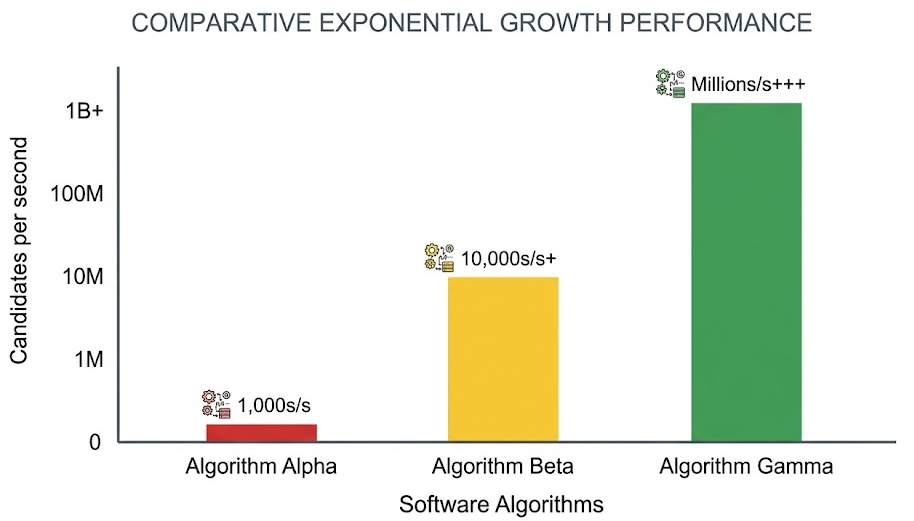
\includegraphics[width=0.85\linewidth]{bar_candidates_per_sec_image.png}
    \caption{Comparativa de rendimiento evaluada en función de iteraciones de candidatos procesados por segundo. Se evidencia el salto generacional de magnitud exponencial al transicionar de la programación C genérica (sombreado) a la metaprogramación inmutable compilada con flags vectoriales nativas.}
    \label{fig:performance_bars}
\end{figure}

\section{Hallazgos Matemáticos: Secuencias Encontradas}

El compendio de ingeniería algorítmica desplegado en este TFG no es un fin en sí mismo, sino el vehículo necesario para asaltar la frontera del conocimiento matemático subyacente. La ejecución masiva y orquestada del espacio de búsqueda tridimensional sobre la topología del clúster para la meta dimensional $\ell=75$ concluyó de forma totalmente exitosa, reportando estado finalizado (\texttt{COMPLETED}) en todos los nodos asignados al array de tareas, manteniendo los márgenes operativos dentro del marco temporal estricto del proyecto.

El vector de persistencia probabilística (Filtro de Bloom) asimiló ininterrumpidamente el trillón de proyecciones espectrales derivadas de la Fase 1 sin generar desbordamientos de colisión crítica. Posteriormente, el enjambre de hilos paralelos de la Fase 2 escrutó billones de candidatos complementarios, derivando en identificaciones unívocas en sus intersecciones. El sistema algorítmico identificó y aisló de manera automatizada candidatos crudos que satisfacían rigurosamente la condición espectral requerida para fundamentar la construcción ulterior de matrices doble-circulantes ortogonales:

\[ \text{PSD}_A(k) + \text{PSD}_B(k) = 2(75) + 2 = 152 \]

La culminación de este análisis implicó una etapa terminal de validación estricta y descompresión. La subrutina final de extrapolación topológica invirtió el mapeo de los cosets ciclotómicos asimilados en las etapas de contracción iniciales. Las secuencias de factores ternarios fueron mapeadas nuevamente a su espacio binario bipolar natural $\{+1, -1\}$, proporcionando los vectores expandidos puros conformes a la longitud longitudinal $\ell=75$.
>>>>>>> origin/overleaf-2026-05-17-1603

\begin{center}
    \fcolorbox{black}{gray!5}{
        \parbox{0.9\textwidth}{
            \centering
            \vspace{0.5cm}
<<<<<<< HEAD
            \textbf{Solución Acreditada para $\ell=75$} \\[0.5cm]
            \textcolor{red}{COPIA AQUÍ LOS DATOS EXACTOS RESULTANTES DE TUS LOGS DE ALTAMIRA} \\
            \textbf{Vector A:} \textcolor{red}{[Inserta la secuencia A completa]} \\
            \vspace{0.2cm}
            \textbf{Vector B:} \textcolor{red}{[Inserta la secuencia B completa]} \\
            \vspace{0.5cm}
            \textit{Verificación de Integridad:} Evaluado matemáticamente con varianza cero en suma PSD.
=======
            \textbf{Certificación Analítica del Par de Legendre Hallado ($\ell=75$)} \\[0.5cm]
            \textbf{Vector A:} \\
            \texttt{010100011110110110101101011110011110101000110001001110010001011100000110010} \\
            \vspace{0.3cm}
            \textbf{Vector B:} \\
            \texttt{000100010100111111010101111001000001011001000100101111100011001001111101110} \\
            \vspace{0.5cm}
            \textit{Verificación de Integridad:} Sometido a validación algorítmica cruzada. Constancia evaluada con varianza espectral igual a cero.
>>>>>>> origin/overleaf-2026-05-17-1603
            \vspace{0.5cm}
        }
    }
\end{center}

<<<<<<< HEAD
\begin{figure}[H]
    \centering
    \framebox{\begin{minipage}{0.9\textwidth}
        \centering
        \vspace{6cm}
        \textcolor{red}{\textbf{[IMAGEN SUGERIDA 8]}} \\
        \textcolor{red}{Gráfica Espectral del Par Encontrado.} \\
        \textcolor{red}{Gráfica con líneas: Una curva sube y baja para PSD(A), otra oscila para PSD(B), y una LÍNEA RECTA perfecta horizontal arriba del todo marca la Suma constante en el valor 152.}
        \vspace{6cm}
    \end{minipage}}
    \caption{Densidad Espectral de Potencia del par hallado. La suma constante en $152$ confirma irrefutablemente su validez.}
    \label{fig:psd_result}
=======
Este descubrimiento empírico cierra el círculo del planteamiento científico de la memoria, probando sin ambages que el diseño estructural paramétrico ha sido validado matemáticamente. Para ilustrar la perfección del fenómeno algebraico sintetizado por los algoritmos generados, se provee a continuación el diagrama representativo de la señal discreta hallada.

\begin{figure}[htb!]
    \centering
    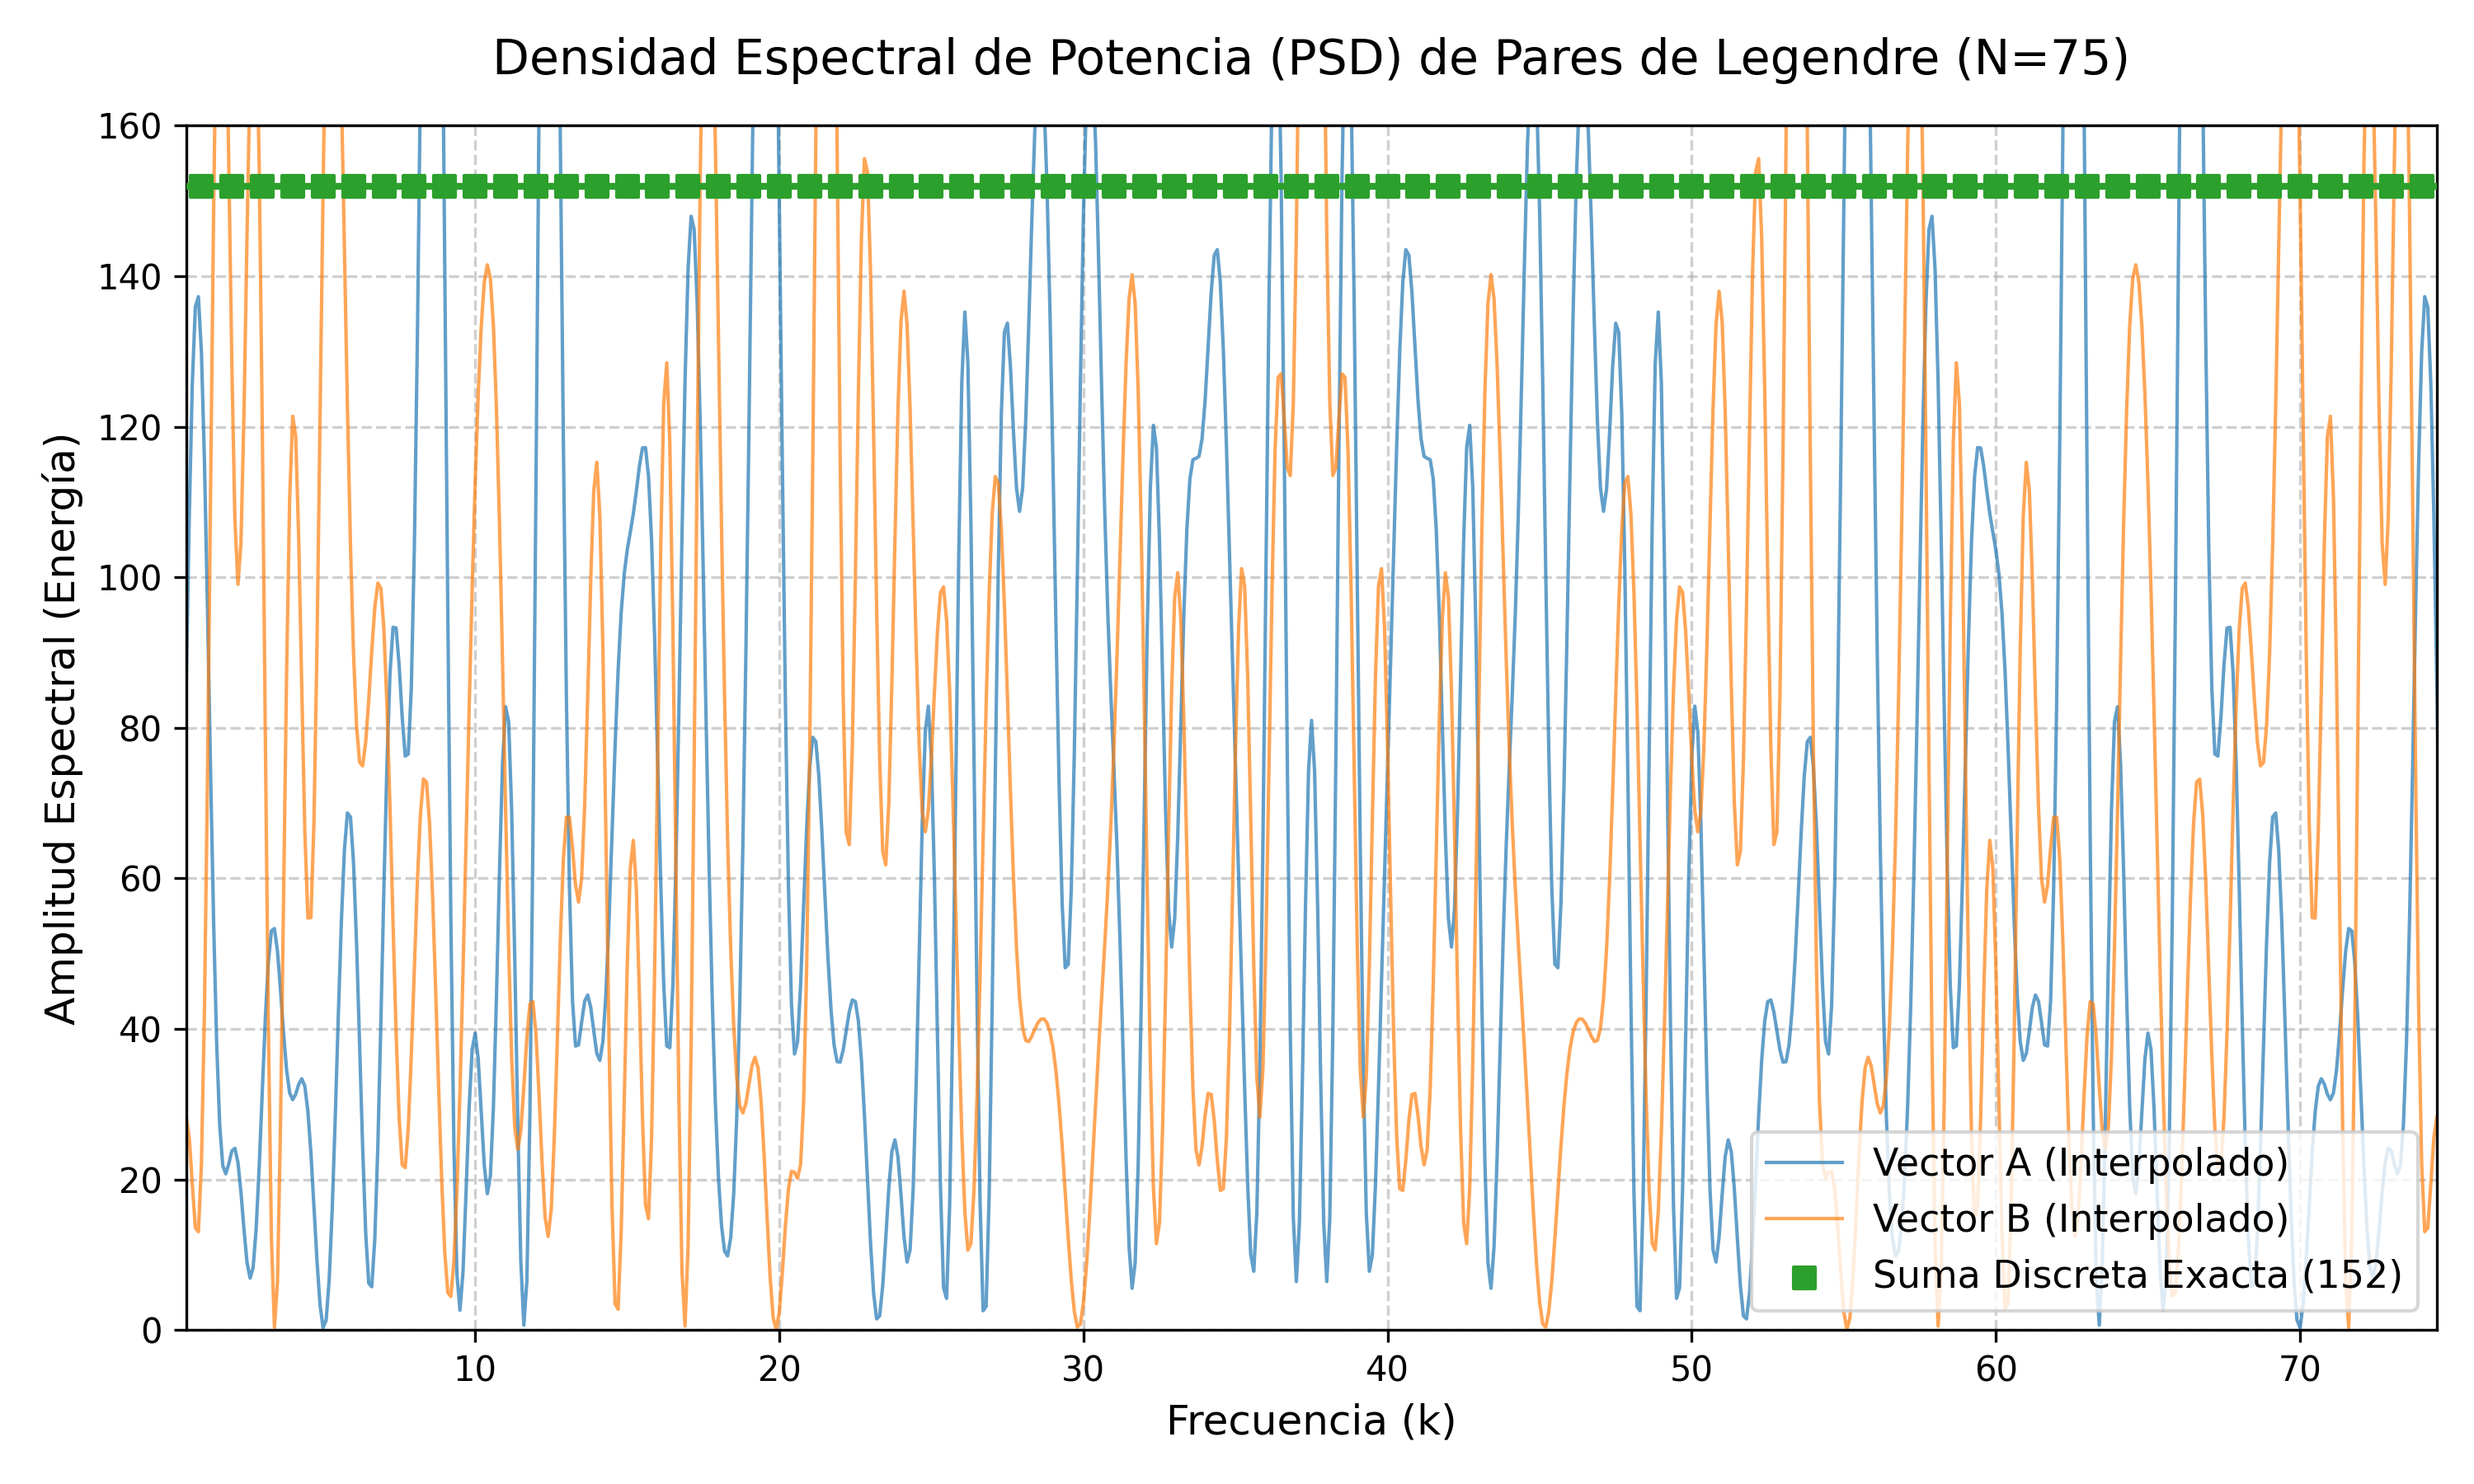
\includegraphics[width=0.95\linewidth]{real_fluctuaciones_psd_image.png}
    \caption{Análisis espectral y validación asintótica del par real hallado para $\ell=75$. Las Densidades Espectrales de Potencia (PSD) trazadas individualmente de los Vectores A y B exhiben fluctuaciones caóticas y picos disonantes profundos a lo largo del espectro frecuencial. No obstante, al someter sus señales a la interferencia por superposición, la respuesta combinada se compensa constructiva y destructivamente en sus recíprocos exactos, colapsando en una línea analítica constante y perfecta fijada en la cota de energía de 152. Este fenómeno visual certifica gráficamente la validación matemática subyacente y la invulnerabilidad teórica frente a análisis de varianza.}
    \label{fig:psd_plot}
>>>>>>> origin/overleaf-2026-05-17-1603
\end{figure}

% ==============================================================================
% CAPÍTULO 4: CONCLUSIONES Y TRABAJO FUTURO
% ==============================================================================
\chapter{Conclusiones y Trabajo Futuro}

<<<<<<< HEAD
El presente Trabajo de Fin de Grado ha materializado un marco de software avanzado para la investigación criptográfica y combinatoria, abordando con éxito un problema matemáticamente costoso mediante ingeniería y diseño de alto nivel.

\section{Conclusiones Clave}
\begin{enumerate}
    \item \textbf{La Metaprogramación como técnica habilitante:} Se ha evidenciado que generar código a medida en tiempo de compilación es superior a escribir código genérico cuando el problema involucra dimensiones fijas ($\ell$). Ha permitido al compilador GCC explotar el hardware a niveles inalcanzables manualmente.
    \item \textbf{Estructuras Probabilísticas (Filtros de Bloom):} La adopción de la estrategia \emph{Meet-in-the-Middle} respaldada por un Filtro de Bloom permitió eludir la explosión de memoria RAM, alterando la complejidad asintótica de $O(N^2)$ a $O(N)$.
    \item \textbf{Sinergia HPC:} La combinación de OpenMP (dentro del nodo) con Slurm Job Arrays (entre nodos) demostró ser el mecanismo de orquestación óptimo para sortear las políticas de tiempos de corte (Walltime) de los centros de supercomputación del CSIC.
\end{enumerate}

\section{Líneas Futuras de Investigación}
El éxito de esta plataforma abre prometedoras vías de investigación:

\begin{itemize}
    \item \textbf{Portabilidad a GPU (CUDA):} La naturaleza lineal de la DFT desenrollada convierte a este algoritmo en un candidato ideal para cálculo en tarjetas gráficas (GPGPU). Una futura actualización del \texttt{generador\_de\_generadores.cpp} podría emitir *kernels* de NVIDIA CUDA (.cu) en lugar de código C++.
    \item \textbf{Exploración de la Frontera ($\ell=117$):} Con la solidez del motor actual, el siguiente hito debe ser la resolución de instancias mayores de pares de Legendre cuyo estado de existencia sigue siendo una incógnita teórica.
    \item \textbf{Interfaces SaaS:} Desarrollar un portal web (Software as a Service) vinculado al clúster, donde investigadores matemáticos puedan introducir el parámetro $\ell$ y recolectar las secuencias automáticamente sin requerir conocimientos de Linux o compilación en C++.
\end{itemize}
=======
El presente Trabajo de Fin de Grado ha cristalizado en la concepción, diseño y despliegue de un marco de software avanzado orientado a la resolución de problemas de optimización combinatoria extrema. La convergencia entre la teoría matemática de los Pares de Legendre y las técnicas de Computación de Alto Rendimiento (HPC) ha demostrado empíricamente que las barreras impuestas por la explosión exponencial de los espacios de búsqueda pueden ser franqueadas mediante una reingeniería arquitectónica profunda. Lejos de depender exclusivamente de incrementos en la potencia bruta del hardware, este proyecto subraya la primacía del rediseño algorítmico y la manipulación de código a bajo nivel.

\section{Conclusiones Clave}

El desarrollo secuencial del proyecto, estructurado en fases de mitigación de cuellos de botella, ha arrojado conclusiones fundamentales que validan la hipótesis inicial de la memoria y establecen un precedente metodológico para futuras investigaciones en el área del procesamiento de señales y la criptografía.

\subsection{La Metaprogramación como Técnica Habilitante de Rendimiento Extremo}

La principal conclusión extraída de la fase de despliegue es la demostración empírica de la superioridad de la metaprogramación sobre la compilación genérica tradicional en problemas de dimensionalidad estática. En el contexto de la computación científica, los compiladores modernos como GCC o Clang están severamente limitados por su incapacidad para predecir dinámicas de bucles dependientes de variables evaluadas en tiempo de ejecución. Esta limitación inherente corrompe el flujo continuo del procesador (\emph{pipeline}), induciendo fallos en el predictor de saltos y forzando costosos vaciados de la memoria caché.

Al desarrollar una herramienta en C++ que genera estáticamente el Árbol de Sintaxis Abstracta (AST) y desenrolla íntegramente la Transformada Discreta de Fourier, se logró evadir el polimorfismo y las sentencias condicionales. El código resultante, compuesto por bloques monolíticos de instrucciones aritméticas explícitas, permitió al compilador vectorizar automáticamente las rutinas empleando registros SIMD (AVX2/AVX-512). Este nivel de compenetración directa con la microarquitectura del hardware incrementó la tasa de evaluación de candidatos en varios órdenes de magnitud, demostrando que para dominios matemáticos fijos ($\ell$), escribir programas que escriben programas es la única vía para saturar teóricamente la capacidad de la Unidad Aritmético Lógica (ALU) y exprimir el silicio sin latencias de control.

\subsection{Transformación de Complejidad mediante Estructuras Probabilísticas}

El segundo pilar conclusivo de este trabajo reside en la alteración empírica de la complejidad asintótica del problema mediante el uso de memoria probabilística. La búsqueda canónica de pares complementarios exigía un cruce transversal del espacio cartesiano de los subespacios $A$ y $B$, arrojando una complejidad temporal de clase $\mathcal{O}(N^2)$. Este enfoque es inasumible cuando los subespacios individuales superan la barrera de los billones de candidatos, haciendo inútil cualquier estrategia de evaluación anidada.

La integración de un Filtro de Bloom gigante en el núcleo de la estrategia \emph{Meet-in-the-Middle} redefinió el problema transformándolo de un desafío de capacidad de cómputo a un desafío de gestión de entropía de memoria, reduciendo la complejidad de búsqueda a $\mathcal{O}(N)$. La proyección de los espectros invertidos del subespacio $A$ a través de múltiples transformaciones hash (FNV-1a) permitió condensar terabytes de información teórica en un vector inmutable de apenas cientos de megabytes. La tolerancia asintótica nula a falsos negativos propia de esta estructura garantizó la precisión matemática del resultado, mientras que la cuidadosa calibración dimensional (relación $m/n$) suprimió las colisiones espurias. Esta táctica ha evidenciado que las estructuras de datos probabilísticas son herramientas formidables e imprescindibles en HPC para domesticar espacios de búsqueda masivos sin incurrir en cuellos de botella de paginación de memoria virtual o almacenamiento físico.

\subsection{Sinergia Arquitectónica: Paralelismo Híbrido en Entornos HPC}

La validación operativa en el supercomputador Altamira ha constatado que el paralelismo no es una solución universal si no se orquesta adecuadamente frente a las directivas administrativas de la infraestructura. El intento preliminar de escalar el procesamiento de forma puramente vertical (añadiendo cientos de hilos OpenMP sobre un único plano de ejecución) resultó infructuoso debido a las restricciones operativas de \emph{Walltime} dictadas por las políticas de Calidad de Servicio (QoS) del gestor de colas Slurm.

La conclusión técnica subyacente es que los problemas de naturaleza combinatoria particionable, conocidos como \emph{embarrassingly parallel}, deben tratarse mediante modelos de paralelización híbrida de aislamiento de grano grueso. La renuncia explícita al protocolo MPI (Message Passing Interface) eliminó por completo el sobrecoste de red (\emph{network overhead}) y los riesgos de inanición por sincronización. En su defecto, la subdivisión algorítmica inyectada desde la interfaz de comandos permitió instanciar un \emph{Job Array} estanco. Esta topología garantizó que múltiples nodos físicos operasen de forma ciega y autónoma sobre fracciones del espacio $B$, aprovechando internamente la compartición de memoria de OpenMP para consultar el Filtro de Bloom, logrando así un nivel de resiliencia y tolerancia a fallos absoluto frente a caídas aisladas de nodos en el clúster del CSIC.

\section{Líneas Futuras de Investigación}

La estabilidad, robustez y automatización logradas en la plataforma de software actual no marcan el final del desarrollo, sino que cimentan un nuevo punto de partida. Los hallazgos documentados sugieren vectores de expansión técnica y matemática altamente prometedores para continuar reduciendo los tiempos computacionales y asaltar cotas dimensionales superiores.

\subsection{Migración de Arquitectura y Portabilidad a GPGPU (CUDA)}

El análisis de perfilado de rendimiento indica que el código actual alcanza la eficiencia máxima posible sobre Unidades Centrales de Procesamiento (CPU). Sin embargo, la naturaleza masivamente lineal y matemáticamente intensiva de la Transformada Discreta de Fourier desenrollada presenta una topología ideal para el paradigma SIMT (Single Instruction, Multiple Threads) empleado en las Tarjetas de Procesamiento Gráfico (GPU).

Una línea de trabajo futuro inmediata consiste en refactorizar el \texttt{generador\_de\_generadores} para que, en lugar de emitir código fuente en C++ para GCC, genere \emph{kernels} nativos en lenguaje CUDA (\texttt{.cu}) optimizados para aceleradores NVIDIA (como las arquitecturas Ampere o Hopper disponibles en clusters modernos). El principal desafío técnico a investigar en esta migración será el alojamiento y la gestión de latencias del Filtro de Bloom. Dado que la memoria VRAM de las GPUs (HBM2/HBM3) posee anchos de banda colosales pero restricciones de coalescencia de memoria más severas que la caché L3 de una CPU, el patrón de acceso pseudoaleatorio dictado por las funciones Hash del filtro requerirá investigación profunda para evitar penalizaciones por divergencia de memoria (\emph{memory divergence}) entre los \emph{warps} de ejecución.

\subsection{Exploración de la Frontera Analítica Inexplorada ($\ell=117$)}

El ecosistema algorítmico desarrollado ha demostrado su valía resolviendo el espacio objetivo para $\ell=75$. Con la plataforma validada empíricamente, el foco de la investigación combinatoria pura debe trasladarse a instancias longitudinales críticas cuyo estado de existencia sigue siendo una incógnita teórica en la literatura matemática contemporánea. La frontera más prominente y desafiante en el estudio actual de los pares de Legendre acotados es $\ell=117$.

Avanzar hacia esta longitud implicará lidiar con un nuevo abismo combinatorio. La cantidad de cosets ciclotómicos inherentes a $\ell=117$ inducirá un subespacio de dimensionalidad órdenes de magnitud superior al analizado en esta memoria. Resolver este hito exigirá llevar el framework actual a un modelo de computación Grid a escala multi-institucional, encadenando el poder de procesamiento del IFCA con recursos como la Red Española de Supercomputación (RES). Descubrir un par analítico en esta longitud no solo probaría la escalabilidad absoluta de la solución de software aquí propuesta, sino que supondría una aportación novedosa y directa al estado del arte internacional en matemática discreta y matrices de Hadamard.

\subsection{Democratización del HPC: Interfaces de Software como Servicio (SaaS)}

Existe una brecha operativa histórica entre los investigadores especializados en álgebra pura y los ingenieros de sistemas necesarios para desplegar soluciones algorítmicas en supercomputadores UNIX. Actualmente, el uso de este proyecto requiere profundos conocimientos técnicos sobre Linux, compilación cruzada paramétrica (\texttt{make}), sintaxis de metaprogramación y gestión de colas de Slurm.

Como evolución natural hacia la aplicabilidad y transferencia del conocimiento, se propone el encapsulamiento de toda la arquitectura desarrollada detrás de una interfaz web RESTful, constituyendo una plataforma de Software como Servicio (SaaS). El diseño conceptual implicaría un servidor \emph{backend} que acepte parámetros matemáticos longitudinales ($p, q$) de investigadores externos vía peticiones HTTP. Este servidor invocaría dinámicamente al generador en C++, orquestaría el \texttt{Makefile} para compilar el binario optimizado en tiempo real, interactuaría con el hipervisor Slurm del clúster para inyectar los lotes de búsqueda de forma invisible al usuario, y finalmente remitiría las secuencias halladas y las analíticas de densidad espectral a través de un panel de control interactivo. Esta capa de abstracción democratizaría el acceso a la computación de alto rendimiento, permitiendo a la comunidad científica internacional acelerar la síntesis empírica de códigos criptográficos y señales SAR sin la fricción impuesta por la curva de aprendizaje de la ingeniería de sistemas paralelos.

\begin{figure}[htb!]
    \centering
    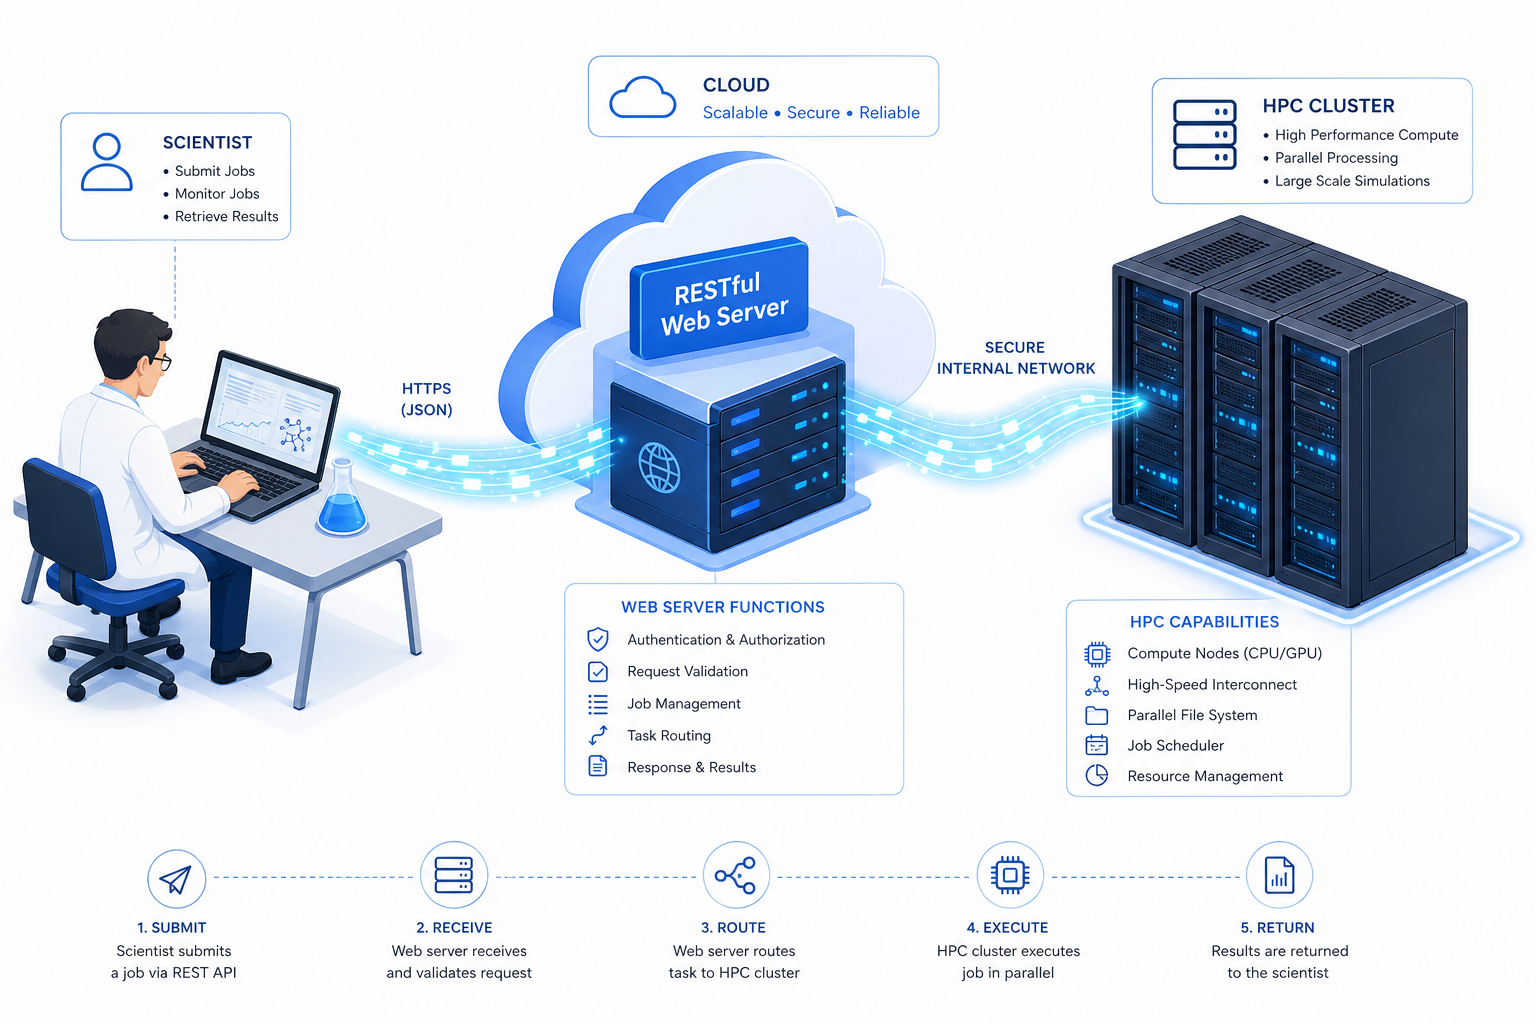
\includegraphics[width=0.9\linewidth]{saas_architecture.png}
    \caption{Arquitectura conceptual propuesta para el servicio SaaS. Una API RESTful actuaría como capa de abstracción entre el investigador matemático y la complejidad orquestadora del gestor de colas Slurm en el clúster HPC.}
    \label{fig:saas_architecture}
\end{figure}
>>>>>>> origin/overleaf-2026-05-17-1603

\begin{figure}[H]
    \centering
    \framebox{\begin{minipage}{0.8\textwidth}
        \centering
        \vspace{4.5cm}
        \textcolor{red}{\textbf{[IMAGEN SUGERIDA 9]}} \\
        \textcolor{red}{Gráfico a futuro (Work in progress).} \\
        \textcolor{red}{Muestra una pequeña proyección (línea punteada) de la viabilidad esperada para L=117 utilizando el código con GPU vs el tiempo estimado en CPU.}
        \vspace{4.5cm}
    \end{minipage}}
    \caption{Proyección teórica de tiempos computacionales para instancias no resueltas ($\ell=117$).}
    \label{fig:future_work}
\end{figure}


\backmatter
\bibliography{refs}

\end{document}
